\documentclass{article}

\usepackage{amsmath}
\usepackage{amsfonts}
\usepackage[left=3cm,right=3cm,top=2.5cm,bottom=2.5cm]{geometry}
\usepackage[sort&compress]{natbib}
\bibliographystyle{apalike}
\usepackage{soul}
\usepackage{url}
\usepackage{circuitikz}
\usepackage{amsthm}
\usepackage[backref=page]{hyperref}
\usepackage{titlesec}
\usepackage{tikz}
\usepackage{array}
\usepackage{caption}
\usepackage{cleveref}
\usepackage[acronym]{glossaries}
\usepackage{subcaption}

\usetikzlibrary{arrows, positioning, arrows.meta}


\newcommand{\xd}{x_{dist}}
\newcommand{\yt}{y_{temp}}
\newcommand{\indep}{\perp \!\!\! \perp}
\newcommand{\refp}[1]{(\ref{#1})}
\newcommand{\degrees}{$^{\circ}$}
\newcommand{\R}{\mathbb{R}}
\newcommand*\circled[1]{\tikz[baseline=(char.base)]{
            \node[shape=circle,draw,inner sep=2pt] (char) {#1};}}

\newtheorem{theorem}{Theorem}
\newtheorem{definition}{Definition}
\newtheorem{corollary}{Corollary}


\title{Active Inference}
\author{Jack Montgomery}
\date{July 2024}

\begin{document}

\begin{titlepage}
    \centering
    \vspace*{1in}
    
    {\LARGE \textbf{Communication in Multi-Agent Reinforcement Learning}}\\[2cm]
    
    {\large \textbf{Jack Montgomery}}\\[0.5cm]
    {\large MNTJAC003}\\[0.5cm]
    {\large MAM4000W - Advanced Topics in Reinforcement Learning}\\ [0.5cm]
    {\large University of Cape Town}\\[2cm]
    
    
\includegraphics[width=0.3\textwidth]{images/UCT_logo_circular_blue_large.png}\\[2cm]
    
    {\large November 2024}\\[2.5cm]
    
    \begin{abstract}

    \end{abstract}
    
\end{titlepage}

\newpage

\tableofcontents

\newpage

\section{Introduction}

Multi-agent systems are ubiquitous in the modern day technological environment. Gives some examples of multi-agent systems. An approach to these intelligent systems is through multi-agent reinforcement learning. Reinforcement learning is build upon the concept of maximising a reward over a certain finite time horizon. In the sense we can consider the two components of this problem as the context or environment in which these systems operate, as well as the solution criteria that is required during the learning.

\

A common technique that has been used in solving some of the issues that arise in Multi-agent reinforcement learning is communication. Communication protocols can serve for many different purposes and generally communication within MARL can be categorised into two sections (with some overlap). The one with solving tasks with communication, otherwise known as Comm-MARL. The other is emergent communication in MARL. Communication within the multi-agent system assists with the problem of non-stationarity, but communication protocols specified a priori require some knowledge of the field that may not be apparent to the designer of the algorithm. This is where the intersetsection of these two paradigms live - where a emergent communication is used to solve a MARL problem. That is ultimately what we will build to in this report.

\

The strategy for this project is to introduce the reader to the results within the single agent reinforcement paradigm that have been fundamental to the architectures proposed for communication within in the multi-agent reinforcement learning problem. Equipped with this context we can then discuss the MARL problem as well as the challenges that we are faced with when scaling from a single agent to multiple in terms of the current tools that we are equipped with from single agent RL. We will then motivate communication as a tool for solving some of these issues as well as discuss some challenges that arise with communication in MARL.

\

The distinction between emergence of language MARL with communication is 

\section{Reinforcement Learning (RL)}

Reinforcement learning, much like machine learning, refers to both a problem as well as a class of solutions \citep{sutton2018reinforcement}. Reinforcement learning problems involve learning what to do - how to map situations to actions - so as to maximise a numerical reward signal. In an essential way they are closed-loop problems because the learning system’s actions influence its later inputs. Moreover, the learner is not told which actions to take, as in many forms of machine learning, but instead must discover which actions yield the most reward by trying them. In the most interesting and challenging cases, actions may affect not only the immediate reward but also the next situation and, through that, all subsequent rewards. These three characteristics - being closed - loop in an essential way, not having direct instructions as to what actions to take, and where the consequences of actions, including reward signals, play out over extended time periods - are the three most important distinguishing features of reinforcement learning problems.


\subsection{Agent - Environment Loop}

Reinforcement learning is a framing of the problem of learning from interactions to achieve a goal. The decision maker (learner) is called the \textit{agent}. The thing it interacts with is called the \textit{environment}. These interact continually, the agent selecting actions and the environment responding to those actions and presenting new situations to the agent. The environment also gives rise to rewards. These are numerical values that the agent seeks to maximise over time.

\

Specifically, the agent and the environment interact over a sequence of discrete time-steps $(t = 1, 2, 3, \hdots)$ At each time-step the agent receives some representation of the environment's state, $S_t \in \mathcal{S}$ where $\mathcal{S}$ is the set of all possible states of the environment, based on that the agent selects an action, $A_t \in \mathcal{A}(S_t)$, where $\mathcal{A}(S_t)$ is the set of all possible actions the agent can take in state $s_t$. In the next time-step, the agent receives a numerical reward $R_{t+1} \in \mathcal{R} \subset \mathbb{R}$, and observes a new state representation $S_{t+1}$. This agent-environment loop is depicted in Figure \ref{fig:agent_environment}. 

\

\begin{figure}
	\centering
	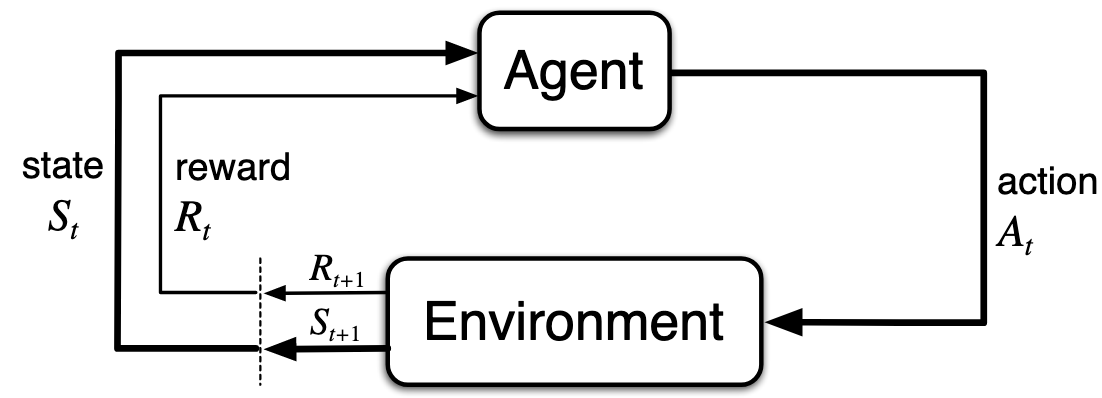
\includegraphics[scale=0.6]{images/agent_environment.png}
	\caption{Image from \citet{sutton2018reinforcement} depicting the agent-environment loop.}
	\label{fig:agent_environment}
\end{figure}

At each time-step the agent implements a mapping from states to a probability distribution over actions. The mapping is called the agent's \textit{policy} and is denoted $\pi_t(a | s)$ which represents the probability $A_t = a$ given $S_t = s$. This mapping fully characterises the agent's behaviour \citep{silver2015rl} so the goal of maximising the total amount of reward the agent receives becomes a problem of finding a policy that maximises the reward the agent receives. 

\subsection{Returns}

%TODO: Need to define an episode

So far we have discussed the learning objective of reinforcement learning informally with the notion that the agent seeks to maximises the rewards it receives over time. Let us denote the sequence of rewards received after time $t$ as $R_{t+1}, R_{t+2}, R_{t+1} \hdots$, we cannot directly effect the reward signal after time $t+1$ from an action at time $t$. Therefore, we seek to maximise the \textit{expected return}, where the return $G_t$ is defined as some function of the rewards sequence. We make the assumption of discounting future rewards - meaning the agent has some bias towards rewards received sooner in the sequence. In particular, it chooses $A_t$ to maximise the \textit{expected discounted return}:

\begin{equation}\label{eq:returns}
	G_t = R_{t+1} + \gamma R_{t+2}+ \gamma^2 R_{t+3} + \hdots = \sum_{k=0}^\infty \gamma^k R_{t + k + 1}
\end{equation}

where $0 \leq \gamma \leq 1$ is called the \textit{discount factor}.

\

Intuitively, a smaller value of $\gamma$ means the agent is more myopic. While a larger value means the agent will be more long-sighted in its selection of actions.

\subsection{Markov Property}

 The state representation that the agent observers, $S_t$, form a chain where $S_{t-1}$ is ``linked'' to $S_t$ through the action taken at time $t - 1$ ($A_{t-1}$). If this chain satisfies the \textit{Markov property} then the reinforcement learning task can be described as a \textit{Markov decision process} (MDP). The \textit{Markov property} means that all information that is needed by the agent can be found in its current state signal. The state signal should include immediate sensations such as sensory measurements, but it can contain much more than that. State representations can be highly processed versions of original sensations, or they can be complex structures built up over time from the sequence of sensations. For example, we can move our eyes over a scene, with only a tiny spot corresponding to the fovea visible in detail at any one time, yet build up a rich and detailed representation of a scene. \citep{sutton2018reinforcement}
 
 \
 
 The Markov property can be stated mathematically for the reinforcement learning problem by considering how an environment may response to an action at time $t$. In general, the reaction may depend on everything that has happened before:
 
 \begin{equation}
 	\mathbb{P}[ R_{t+1} = r, \ S_{t+1} = s' | S_0, A_0, \hdots, S_t, A_t]
 \end{equation}
 
 If we assume that chain of state signals does obey the Markov property, then the expression of the reaction of the environment can be simplified to:
 
 \begin{equation}
 	p(s', r | s, a) = \mathbb{P}[ R_{t+1} = r, \ S_{t+1} = s' | S_t, A_t]
 \end{equation}
 
 The Markov property is important in reinforcement learning because decisions and values are assumed to be a function only of the current state. In order for these to be effective and informative, the state representation must be informative. \citep{sutton2018reinforcement}

%\subsection{RL Problem}
%
%The fundamental problem that we consider in reinforcement learning is the learn an optimal policy that chooses actions to achieve some objective, which can be the sum of the discounted expected future rewards. RL solutions seek to find this policy through repeated interaction with the environment. 
%
%
%
%The problem statement and proposed solution need more clarity. Specifically, what is a sequential decision process, what could be a solution to this and how does one learn it through repeated interaction. This first section of the paper aims to define and answers each of these questions.
%
%\
%
%A sequential decision process is defined by an agent that makes decisions over multiple time steps within an environment to achieve a specified goal. In each time step, the agent receives an observation from the environment and chooses an action. In a fully observable setting, as we assume in this chapter, the agent observes the full state of the environment; but in general, observations may be incomplete and noisy. Given the chosen action, the environment may change its state according to some transition dynamics and send a scalar reward signal to the agent. \citep{albrecht2024marl} (INSERt IMAGE)
%
%\
%
%A solution to the decision process is an optimal decision policy for the agent, which chooses actions in each state to achieve some specified learning objective. Typically, the learning objective is to maximise the expected return for the agent in each possible state.1 The return in a state when following a given policy is defined as the sum of rewards received over time from that state onward. Thus, RL assumes that the goal in the decision process can, in principle, be framed as the maximisation of expected returns.
%
%\
%
%Finally, RL algorithms learn such optimal policies by trying different actions in different states and observing the outcomes. This way of learning is sometimes described as ``trial and error'' since the actions may lead to positive or negative outcomes that are not known beforehand and, therefore, must be discovered by trying the actions. A central problem in this learning process, often called the exploration-exploitation dilemma, is how to balance exploring the outcomes of different actions versus sticking with actions that are currently believed to be best. Exploration may discover better actions but can accrue low rewards in the process, while exploitation achieves a certain level of returns but may not discover the optimal actions.

\subsection{Markov decision processes}

If the set of states and the set of actions are finite then the MDP is called a \textit{finite Markov decision process}. This is the foundational framework for reinforcement learning problems. 

\

A finite MDP is defined by its set if states $\mathcal{S}$, and the set of actions, $\mathcal{A}$. As well as by the one step dynamics of the environment. Given any state ($s \in \mathcal{S}$) and action ($a \in \mathcal{A}$) the probability of each possible pair of next states ($s' \in \mathcal{S}$) and reward ($r \in \mathcal{R}$) is denoted:

\begin{equation}
	p(s', r | s, a) = \mathbb{P}[ R_{t+1} = r, \ S_{t+1} = s' | S_t, A_t]
\end{equation}

These quantities fully define a finite MDP.

\subsection{Value Functions}

Almost all solution to reinforcement learning problems involve some estimation of the ``goodness'' of states. Intuitively this makes sense as we need some understanding of the reward dynamics of the environment before we could hope we find a policy that maximises these rewards. The ``goodness'' is measured in terms of discounted expected future returns (\ref{eq:returns}) and is encapsulated in the \textit{value function}. Of course the rewards the agent can expect to receive in the future depend on what actions it will take. Accordingly, value functions are defined with respect to particular policies. Formally, the value function is expressed as:

\begin{equation}\label{eq:value_function}
	v_\pi(s) = \mathbb{E}_\pi\left[ G_t \middle| S_t = s \right] = \mathbb{E}_\pi\left[ \sum_{k=0}^\infty \gamma^t R_{t + k + 1} \middle| S_t = s \right]
\end{equation}

Similarly, we define the value of taking action $a$ in state $s$ under a policy $\pi$, denoted $q_\pi(s, a)$, as the expected return starting from $s$, taking the action $a$, and thereafter following policy $\pi$:

\begin{equation}
	q_\pi(s, a) = \mathbb{E}_\pi \left[ G_t  \middle| S_t = s, A_t = a\right] = \mathbb{E}_\pi \left[ \sum_{k=0}^\infty R_{t + k + 1} \middle| S_t = s, A_t = a\right]
\end{equation}

We will call $v_\pi$ the value of a state and the $q_\pi$ the q-value of a state-action pair.

\

The functions $v_\pi$ and $q_\pi$ can be estimated from experience. For example, if an agent follows policy $\pi$ and maintains an average, for each state encountered, of the actual returns that have followed that state, then the average will converge to the state’s value, $v_\pi(s)$, as the number of times that state is encountered approaches infinity. If separate averages are kept for each action taken in a state, then these averages will similarly converge to the action values, $q_\pi(s, a)$. We call estimation methods of this kind \textit{Monte Carlo methods} because they involve averaging over many random samples of actual returns. Of course, if there are very many states, then it may not be practical to keep separate averages for each state individually. Instead, the agent would have to maintain $v_\pi$ and $q_\pi$ as parameterised functions and adjust the parameters to better match the observed returns. This can also produce accurate estimates, although much depends on the nature of the parameterised function approximator. These methods will be covered in Section \ref{sec:deep_rl}.

\

A fundamental property of value functions used throughout reinforcement learning and dynamic programming is that they satisfy particular recursive relationships. For any policy $\pi$ and any state $s$, the following consistency condition holds between the value of s and the value of its possible successor states:

\begin{equation}\label{eq:bellman_equation}
	v_\pi(s) = \mathbb{E}_\pi [ G_t | S_t = s ] = \sum_a \sum_{s', r} p(s', r | s, a) \left[ r + \gamma v_\pi(s') \right]
\end{equation}

This expression is known as the Bellman equation for $v_\pi$. It expresses a relationship between the value of a state and the values of its successor states. We will see that this expression forms the basis of a number of techniques to compute, approximate and learn $v_\pi$.

\subsection{Optimal Value Functions}

As mentioned, solving a reinforcement learning problem means finding a policy that maximises the rewards over time. For finite MDPs, we can precisely define an optimal policy in the following way. Value functions define a partial ordering over policies. A policy $\pi$ is defined to be better than or equal to a policy $\pi'$ if its expected return is greater than or equal to that of $\pi'$ for all states. In other words, $ \pi \geq \pi' \iff v_\pi(s) \geq v_{\pi'}(s), \ \forall s \in S$. There is always at least one policy that is better than or equal to all other policies. \citep{sutton2018reinforcement} This is an \textit{optimal policy}. Though this policy may not be unique, we will denote the all optimal policies by $\pi_*$. They share the same value function, called the optimal value function, denoted $v_*$, and defined as:

\begin{equation}
	v_*(s) = \max_{\pi} v_\pi(s), \ \forall s \in \mathcal{S}
\end{equation}

Similarly, optimal policies share the same optimal q-value function, $q_*$:

\begin{equation}
	q_*(s, a) = \max_{\pi} q_\pi(s, a), \ \forall s \in \mathcal{S} \ \forall a \in \mathcal{A}(s)
\end{equation}

 We can also note that we can recover the optimal value function from the q-value function by marginalising over all possible actions:

\begin{equation}
	v_*(s) = \max_{a \in \mathcal{A}(s)} q_{\pi_*}(s, a)
\end{equation}


We have defined optimal value functions and optimal policies. Clearly, an agent that learns an optimal policy has done very well, but in practice this rarely happens. For the kinds of tasks in which we are interested, optimal policies can be generated only with extreme computational cost. However, a well-defined notion of optimality organises the reinforcement learning approaches described in this report and provides a way to understand the theoretical properties of various learning algorithms, but it is an ideal that agents can only approximate to varying degrees.

\subsection{Joint learning problem}

What we have described using value function is a measure of the goodness of an agent's policy. However, we aim for this agent to have (or approach) an optimal policy described in the previous section. These represent two different problems. To learn the rewards dynamics of an environment given a policy, as well as learn what policy maximises rewards within that finite MDP. Solving this problem means that an agent could be dropped into an environment, learn how the environment works and solve the environment by finding the optimal policy. This is the lofty, but fundamental goal of reinforcement learning.

\

The process of learning the value function given a policy is known as \textit{policy evaluation}, while the process of making that policy better is known as \textit{policy improvement}. The good news is that these processes are not exclusive of one another - if an agent has a good understanding of the reward landscape of an MDP, then it becomes easier to construct a good policy to solve that MDP.

\

If we were to consider a situation where the agent had a perfect model of the environmental state and reward dynamics, the simplest policy they can employ is a \textit{greedy policy} - meaning they always choose the action that obtains the highest value in the next state. In our assumption, we do not have a perfect model of the environment, therefore we need to continually explore the environment for alternative paths to our objective. This is known as a $\varepsilon$-greedy policy. This is written formally as:

\begin{equation}
	\pi(a | s) = \begin{cases}
		1 - \epsilon + \frac{\epsilon}{|\mathcal{A}|} & \text{if } a = \arg \max_{a'} Q(s, a') \\
		\frac{\epsilon}{|\mathcal{A}|} & \text{otherwise}
	\end{cases}
\end{equation}

This is a simple mechanism to ensure continual exploration in the MDP, that works surprisingly well. The most useful property of employing an $\varepsilon$-greedy policy is that for any $\varepsilon$-greedy policy $\pi$, the $\varepsilon$-greedy policy $\pi'$ with respect to $q_\pi$ is an improvement, $v_{\pi'}(s) \geq v_\pi(s)$:

\begin{equation}
\begin{aligned} 
    q_\pi\left(s, \pi^{\prime}(s)\right) 
    &= \sum_{a \in \mathcal{A}} \pi^{\prime}(a \mid s) q_\pi(s, a) \\
    &= \frac{\varepsilon}{m} \sum_{a \in \mathcal{A}} q_\pi(s, a) + (1 - \varepsilon) \max_{a \in \mathcal{A}} q_\pi(s, a) \\
    &\geq \frac{\varepsilon}{m} \sum_{a \in \mathcal{A}} q_\pi(s, a) 
        + (1 - \varepsilon) \sum_{a \in \mathcal{A}} \frac{\pi(a \mid s) - \frac{\varepsilon}{m}}{1 - \varepsilon} q_\pi(s, a) \\
    &= \sum_{a \in \mathcal{A}} \pi(a \mid s) q_\pi(s, a) = v_\pi(s)
\end{aligned}	
\end{equation}

What this means in the context of our joint learning problem is that we can use the $\varepsilon$-greedy algorithm to ensure exploration and allow the agent to learn the reward landscape in the MDP, as well as improve its policy. The idea is that these two processes will eventually converge to $q_*$ and $\pi_*$ the optimal q-value function and optimal policy respectively. This is visualised in Figure \ref{fig:eval_improvement}.

\begin{figure}
	\centering
	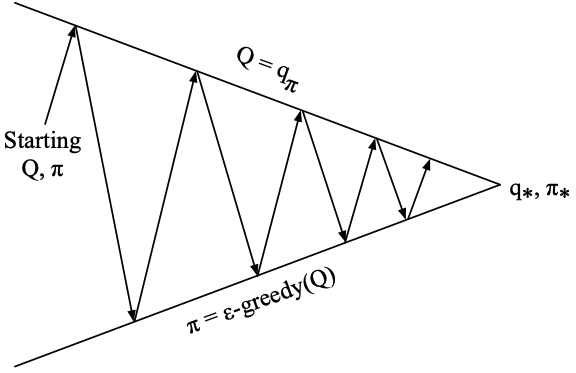
\includegraphics[scale=0.4]{images/eval_improve.png}
	\caption{Image from \citet{silver2015rl} demonstrating the process of policy improvement and policy evaluation using an $\varepsilon$-greedy policy that ideally converges to the optimal policy and q-value function.}
	\label{fig:eval_improvement}
\end{figure}

\subsection{Model-Based vs Model-Free}

In general, reinforcement learning algorithms can be considered as model-free or model-based, through this line may sometimes be blurry. In model-based reinforcement learning the agent is learning a representation of the environmental dynamics, while in model-free reinforcement learning the agent is only tasked with learning the reward landscape in state-action space.

\

A model in this case would be a representation of how the environmental states will react to action taken by the agent. In this, an agent would be able to query its own model of the environment with a chain of possible actions to then to able to plan multiple time-steps into the future. Though, the model-free techniques have the future rewards encoded into their value estimates, model-based reinforcement learning has found much success within the field. \citep{moerland2022model} In this report we will be exclusively focussing on model-free algorithms.

\subsection{Example: Tabular q-learning}

To illustrate a solution to a MDP with reinforcement learning, we will consider the Frozen Lake environment from OpenAI Gymnasium \citep{kwiatkowski2024gymnasium}. In this environment, an agent must navigate from a starting position to a goal position on a frozen grid, avoiding holes that would end the episode prematurely. The environment consists of a \(4 \times 4\) grid-world with the following specifications:

\begin{itemize}
    \item \(\mathcal{S} = \{1, 2, \dots, 16\}\): The set of 16 possible states, each representing a unique cell on the grid.
    \item \(\mathcal{A} = \{\text{RIGHT}, \text{DOWN}, \text{LEFT}, \text{UP}\}\): The set of 4 possible actions.
    \item Rewards, \(\mathcal{R}\):
    $$
    \mathcal{R} = \begin{cases}
        1, & \text{if the agent reaches the goal} \\
        0, & \text{otherwise}
    \end{cases}
    $$
\end{itemize}

\begin{figure}
	\centering
	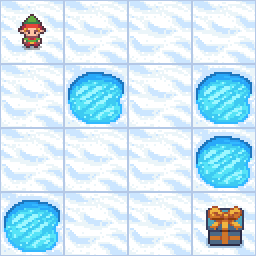
\includegraphics[scale=0.5]{images/frozen_lake_frame.png}
	\caption{Screenshot from FrozenLake \citep{kwiatkowski2024gymnasium}}
	\label{fig:frozen_lake}
\end{figure}

We will be using a tabular q-learning with a $\varepsilon$-greedy policy in order to solve this environment. What tabular q-learning requires is the storage of state-action values, in other words, we require a table of q-values. From the specifications of the environment, this will be a matrix of dimension $16 \times 4$. As depicted in Figure \ref{fig:eval_improvement} we require some starting point for our q-values, which we choose to be $0$. 

\

Through experience, we seek to learn what actions we should take in particular states of the environment. Therefore, we define the following update equation based on the Bellman equation (for our q-value estimate) for a state-action pair:

\begin{equation}\label{eq:q_update}
    q(s_t, a_t) \leftarrow r_t + \gamma  \max_{a' \in \mathcal{A}(s_{t+1})} q(s_{t+1}, a')
\end{equation}

This is the fundamental equation in the q-learning algorithm.

\

To demonstrate the learning of done by the agent we can plot a heat map of each state in the environment based on the q-value of the most rewarding action. Intuitively, we should see a heat map the depicts states near the reward state with a higher maximum value action. This is depicted in Figure \ref{fig:frozen_lake_q_learning}.

\begin{figure}[htp]
    \centering
    \begin{subfigure}{0.3\textwidth}
        \centering
        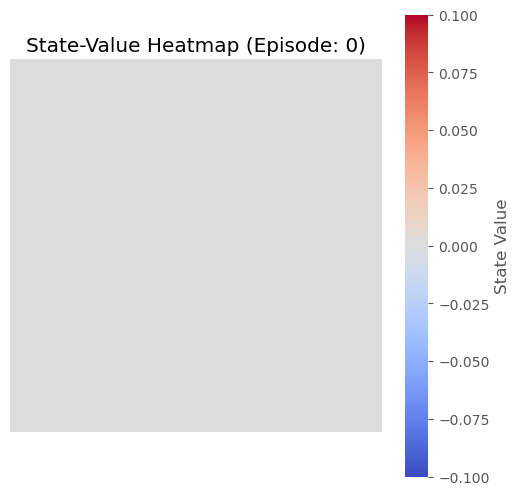
\includegraphics[width=\linewidth]{images/frozen_0.png}
        \caption{}
        \label{fig:t0}
    \end{subfigure}
    \hfill
    \begin{subfigure}{0.3\textwidth}
        \centering
        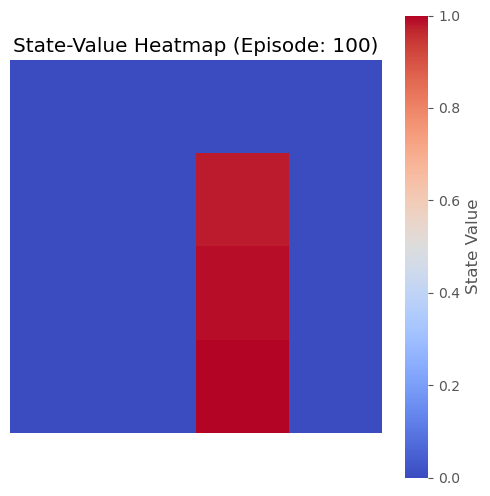
\includegraphics[width=\linewidth]{images/frozen_100.png}
        \caption{}
        \label{fig:t100}
    \end{subfigure}
    \hfill
    \begin{subfigure}{0.3\textwidth}
        \centering
        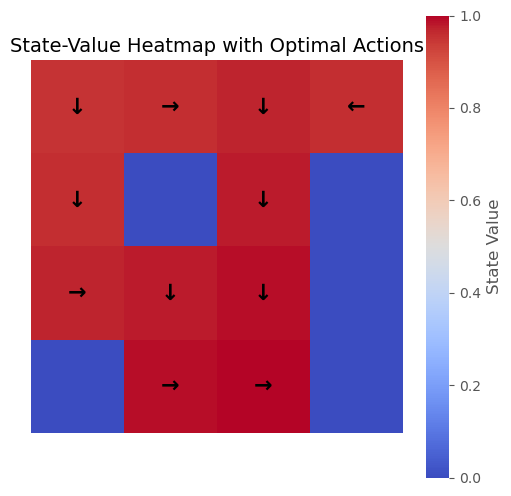
\includegraphics[width=\linewidth]{images/frozen_with_actions.png}
        \caption{}
        \label{fig:t200}
    \end{subfigure}
    
    \caption{Maximum action value state map of the frozen lake environment using tabular q-learning with exponentially decaying $\varepsilon$-greedy policy before episode 0 (\ref{fig:t0}), 100 (\ref{fig:t100}) and 200 (\ref{fig:t200}). The final plot (\ref{fig:t200}) has the optimal action indicated on the state with an arrow in the direction of that action. }
    \label{fig:frozen_lake_q_learning}
\end{figure}

\

In Figure \ref{fig:frozen_lake_q_learning}, we observe that through the random exploration of the environment the agent is able to find a corridor of high value actions seen in Figure \ref{fig:t100}. After an additional 100 episodes, the value of the actions in this corridor have been propagated throughout the environment, apart from the states that contain the obstacles. The difficulty of this environment is the sparsity of the rewards. The agent is only rewarded when getting to the goal, meaning that the only way the agent can make good decisions early is by bootstrapping the values that have been learned during the episodes. 

\

Further, we can see that the greedy action in each state depicted in Figure (\ref{fig:t200}) describe a path through the environment that is optimal to get to the desired reward location, therefore we can say that this tabular q-learning algorithm has indeed solved this MDP with no prior knowledge about the environment or policy needed.

\subsection{Deep RL Algorithms}\label{sec:deep_rl}

The problem with the approach of tabular learning is that the table that we use to store our estimates of the q-values soon becomes intractable as the state space and action space grow. A solution that has been used to solve this problem is using so-called ``deep'' methods. What this means is that we use neural networks as function approximators. What exactly these networks approximates can be the policy, q-values or values of the states. The salient point is that using these neural networks is that we no longer store large tables of data that are refined using experience with the environment - we use this experience to refine the set of parameters of our neural network which means the storage space of the machinery we use to solve these reinforcement learning problems does not grow significantly with increases to the state or action space.

\subsubsection{Deep Q-Learning}

The foundational work in the field of deep reinforcement learning was done by \citet{mnih2013playing}, in which they proposed the Deep Q-Network (DQN). While previous approaches attempted to use non-linear function approximations for reinforcement learning \citep{tsitsiklis1996temporal}, this work represented the first instance of a neural network effectively solving a complex problem in the domain of reinforcement learning.

\

The challenge with using neural networks for Q-learning lies in the fact that the agent must learn both the dynamics of the environment and the policy that maximizes reward simultaneously. This results in a moving target problem. With non-linear function approximators like neural networks, this can introduce instability during training, as the objective surface continually shifts. In standard supervised learning, the objective function remains constant during optimization; however, in reinforcement learning, the objective surface evolves as the agent updates its estimates of the environment. This makes it difficult to converge on an optimal solution.

\

To address this instability, \citet{mnih2013playing} introduced two key mechanisms in DQN:

\begin{enumerate}
	\item \textbf{Target Network}: Instead of using the Q-network directly to update itself, DQN maintains a separate target network that is a periodically frozen copy of the Q-network. The Q-network is used to select actions, while the target network generates stable Q-value estimates, providing a more consistent objective surface. The target network is updated less frequently than the Q-network, effectively reducing oscillations and stabilising the learning process.
	\item \textbf{Experience Replay}: Rather than using consecutive experiences from the environment for training (which introduces correlations between data points), DQN stores past experiences in a replay buffer. During training, experiences are sampled randomly from this buffer, breaking the temporal correlation and ensuring that the training data is more representative of the agent's overall experience. This process also improves sample efficiency, as each experience is reused multiple times, maximizing learning from each interaction with the environment.

\end{enumerate}

The loss function used to update the Q-network in DQN is based on the temporal difference (TD) error, given by:

\begin{equation}
L(\theta) = \mathbb{E}_{(s, a, r, s') \sim D} \left[ \left( y - Q(s, a; \theta) \right)^2 \right],
\end{equation}

where $y = r + \gamma \max_{a'} Q(s', a'; \theta_\text{target})$ is the target value computed using the target network parameters $\theta_\text{target}$, and $D$ is the replay buffer. The goal is to minimize this TD error by updating the Q-network parameters $\theta$, encouraging the network to improve its estimates of the Q-values over time.

\

These innovations allowed DQN to achieve breakthrough performance on challenging tasks, such as playing Atari games from pixel input, which had previously been out of reach for reinforcement learning algorithms.

\subsubsection{Deep Recurrent Q-Learning}\label{sec:drqn}

While DQN demonstrated remarkable results, it assumes that the environment is fully observable, meaning the agent has access to all relevant information about the current state. However, in many real-world environments, the agent operates under partial observability, where only part of the information about the current state is available at any given time. For example, an agent navigating through a maze may not know its exact location without a full view of the environment.

\

To address this limitation, \textbf{Deep Recurrent Q-Learning (DRQN)} was introduced \citep{hausknecht2015deep}. DRQN combines the structure of DQN with recurrent neural networks (RNNs), allowing the agent to maintain an internal memory of previous observations, which can be used to infer hidden aspects of the state. By incorporating a recurrent layer, such as a Long Short-Term Memory (LSTM) or Gated Recurrent Unit (GRU), DRQN can process sequences of observations over time, making it better suited to environments with partial observability.

\

The Q-value estimate in DRQN is modified as follows:

\begin{equation}
Q(s_t, a_t; \theta, h_{t-1}) = f(s_t, h_{t-1}; \theta),
\end{equation}

where $h_{t-1}$ is the hidden state from the previous time step, carrying information about the sequence of past observations, and $f$ is the RNN function (e.g., LSTM or GRU) parameterized by $\theta$. The hidden state $h_{t-1}$ is updated at each time step, allowing DRQN to form a context over time and make informed decisions in partially observable environments.

\

The DRQN training process is similar to DQN, including the use of experience replay and a target network to stabilise training. However, the replay buffer in DRQN is adapted to store entire sequences (trajectories) rather than individual transitions, enabling the RNN to learn temporal dependencies. The training loss is computed by sampling sequences from the replay buffer and back-propagating the error through time, allowing the agent to learn from temporally-extended experience.

\

DRQN extends the capabilities of DQN to a wider range of environments by equipping the agent with a memory mechanism. This allows it to excel in tasks where full observability is not guaranteed, making it more applicable to complex, real-world scenarios.

\subsubsection{Actor-Critic} 

Methods of Q-learning form part of value-based learning, where the task of the agent is to estimate the reward landscape of the state-action pairs, also known as the Q-values, for a given environment. From these estimates, a policy can be derived, often using an $\varepsilon$-greedy approach, which balances exploration and exploitation by occasionally choosing random actions. In contrast, \textbf{policy-based methods} seek to learn the optimal policy directly within a Markov Decision Process (MDP) by parameterising the policy itself rather than relying on value estimates of state-action pairs.

\

The fundamental algorithm in this category is \textbf{REINFORCE} \citep{williams1992simple}. This is a Monte-Carlo-based method, meaning that learning takes place after completing an entire trajectory (episode). At the end of each trajectory, the cumulative returns $G_t = \sum_{k=0}^{\infty} \gamma^k R_{t+k+1}$ for a given action in each state encountered are fully observed. Here, $\gamma$ is the discount factor, which determines the importance of future rewards relative to immediate rewards.

\

The REINFORCE algorithm adjusts the parameters of the policy $\pi_\theta(a|s)$ by increasing the probability of actions that led to high returns and decreasing it for those leading to low returns. Mathematically, this adjustment is achieved by updating the policy parameters $\theta$ in the direction of the gradient of the expected return:

\begin{equation}
\theta \leftarrow \theta + \alpha \nabla_\theta J(\theta),
\end{equation}

where $\alpha$ is the learning rate, and $J(\theta) = \mathbb{E}_{\pi_\theta} [G_t]$ represents the expected return under the policy $\pi_\theta$. Using the \textbf{policy gradient theorem} \citep{sutton1999policy}, this gradient can be expressed as:

\begin{equation}
\nabla_\theta J(\theta) = \mathbb{E}_{\pi_\theta} \left[ G_t \nabla_\theta \log \pi_\theta(a_t | s_t) \right].
\end{equation}

In practice, this expectation is estimated from a single trajectory by applying the following update rule:

\begin{equation}
\theta \leftarrow \theta + \alpha G_t \nabla_\theta \log \pi_\theta(a_t | s_t).
\end{equation}

This adjustment rule intuitively increases $\pi_\theta(a_t | s_t)$ when the return $G_t$ is high (reinforcing the likelihood of actions that yield high rewards) and decreases it when $G_t$ is low. The reliance on a Monte Carlo approach (using full trajectories) makes REINFORCE unbiased but often results in high variance in the updates, which can make convergence slower. Techniques such as using \textbf{baselines} can be introduced to reduce this variance, where a baseline $b(s_t)$ is subtracted from $G_t$ to adjust the update as follows:

\begin{equation}
\theta \leftarrow \theta + \alpha (G_t - b(s_t)) \nabla_\theta \log \pi_\theta(a_t | s_t).
\end{equation}

This baseline, often set to an estimate of the state value $V(s_t)$, helps centre the updates, making the learning process more stable by only reinforcing actions that perform above the baseline. This is known as the critic.

\

Actor-critic methods maintain two neural networks. The actor maps the observations into the probability distribution over actions and can be understood as the policy network. The critic is an estimate of the rewards of the state action pairs state-action. The critic is then trained on the rewards obtained from the environment, similarly to how a DQN is trained. And the actor is trained based on the temporal-difference update generated by the critic network. 

\subsubsection{Proximal Policy Optimisation (PPO)}

While actor-critic methods offer an effective way to combine the benefits of both value-based and policy-based learning, they can suffer from instability. In particular, if the policy updates are too large, the agent's behaviour can oscillate, leading to divergence rather than convergence. This instability arises because a large update can significantly change the policy, moving it too far from the policy that generated the value estimates, thereby making the value function inaccurate for the updated policy.

\

To address this issue, a regularisation approach known as \textbf{Trust Region Policy Optimisation (TRPO)} was introduced \citep{schulman2015trust}. TRPO limits the update step size to constrain how far the new policy deviates from the old policy, which reduces the risk of instability. This is achieved by optimising a surrogate objective function while enforcing a constraint on the Kullback-Leibler (KL) divergence between the old and new policies. The TRPO objective can be expressed as:

\begin{equation}
\max_\theta \mathbb{E}_{s \sim \pi_\text{old}} \left[ \frac{\pi_\theta(a|s)}{\pi_\text{old}(a|s)} A^{\pi_\text{old}}(s, a) \right],
\end{equation}

subject to the constraint:

\begin{equation}
\mathbb{E}_{s \sim \pi_\text{old}} \left[ D_\text{KL}(\pi_\text{old} \| \pi_\theta) \right] \leq \delta,
\end{equation}

where $A^{\pi_\text{old}}(s, a)$ is the advantage function calculated using the old policy $\pi_\text{old}$, and $\delta$ is a threshold that restricts the KL divergence to maintain a trust region around the old policy. This constraint limits drastic changes in the policy, ensuring smoother updates and more stable learning.

\

While effective, TRPO can be complex to implement due to its reliance on a second-order optimisation technique to enforce the KL constraint. To simplify this, \textbf{Proximal Policy Optimisation (PPO)} \citep{schulman2017proximal} was developed. PPO uses a modified objective function that replaces the strict KL constraint with a clipped surrogate objective, making the algorithm both simpler to implement and computationally efficient while retaining the stability benefits of TRPO.

PPO’s objective function is given by:

\begin{equation}
L^{\text{CLIP}}(\theta) = \mathbb{E}_{s \sim \pi_\text{old}, a \sim \pi_\theta} \left[ \min \left( r(\theta) A^{\pi_\text{old}}(s, a), \text{clip}(r(\theta), 1 - \epsilon, 1 + \epsilon) A^{\pi_\text{old}}(s, a) \right) \right],
\end{equation}

where the probability ratio $r(\theta)$ is defined as:

\begin{equation}
r(\theta) = \frac{\pi_\theta(a|s)}{\pi_\text{old}(a|s)}.
\end{equation}

The clipping function limits the change in $r(\theta)$ within the interval $[1 - \epsilon, 1 + \epsilon]$, where $\epsilon$ is a hyper-parameter. By applying this clipping, PPO discourages excessively large updates, thus providing a balance between exploration and policy stability. The objective function ensures that if the update moves the policy ratio outside of this range, the advantage term is effectively set to zero, preventing excessive updates.

\

In practice, PPO achieves a robust performance by iteratively sampling trajectories, estimating the advantage values using the critic, and optimising the clipped objective to update the actor network. The simplicity and effectiveness of PPO have made it a popular choice for many reinforcement learning tasks where stability and performance are critical considerations.

\section{Multi-Agent Reinforcement Learning (MARL)}

While single-agent reinforcement learning has achieved significant success, many real-world problems involve multiple interacting agents, which are collectively referred to as \textit{multi-agent systems}. These systems require agents to collaborate or compete to achieve complex objectives. For instance, in smart power grids, agents coordinate to manage electricity distribution by synchronising generators, storage, utilities, and consumers, enabling the integration of renewable energy sources. In disaster rescue scenarios, autonomous robots work together to map disaster areas, locate survivors, and deliver essential supplies. In this chapter, we will extend the tools developed for single-agent reinforcement learning to tackle the unique challenges of multi-agent systems, exploring methods for effective coordination, competition, and resource sharing among agents.

\subsection{Multi-agent system}

A multi-agent system consists of an \textit{environment} and \textit{agents} that interact in the environment to achieve some goal. This is similar to agent agent-environment loop that was described in the first section only that not the combination of all $n$ agents within the environment will affect the underlying state. This loop is described in Figure \ref{fig:agents_environment_loop}. 

\begin{figure}
	\centering
	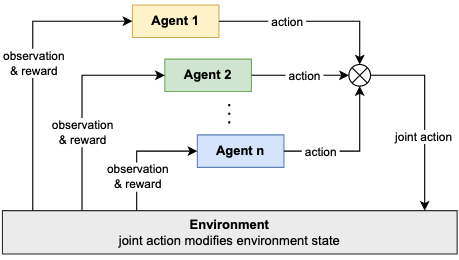
\includegraphics[scale=0.6]{images/multiple_agent_environment.png}
	\caption{Image from \citet{albrecht2024marl} describing the agents-environment loop at play in multi-agent systems.}
	\label{fig:agents_environment_loop}
\end{figure}

\

The collection of states, actions, observations, and rewards are formally defined within \textit{game models}. Different types of game models exist, and we introduce common game models used in MARL in Section \ref{sec:game_models}, including  stochastic games, and partially observable stochastic games. A solution for a game model consists of a set of policies for the agents that satisfies certain desired properties. The exact properties that are desired are formally solution concepts, some common forms of solution concepts are described in Section \ref{sec:solution_concepts}.

\subsection{Game models}\label{sec:game_models}

In a very similar fashion to how our description of the reinforcement learning task then fed into our description of a Markov decisions process, with the assumption of the Markov property on the chain of states within the tasks. We will too be placing a multi-agents systems into process frameworks that are called game models. 

\

A multi-agent system can be formalised in many different ways \citep{oliehoek2016concise} depending on whether the environment is fully observable, how agents' goals are correlated, or whether communication and coordination between agents are allowed. The partially observable stochastic game (POSG) \citep{hansen2004dynamic} is defined by a tuple $\left\langle\mathcal{I}, \mathcal{S}, \rho^0,\left\{\mathcal{A}_i\right\}, P,\left\{\mathcal{O}_i\right\}, O,\left\{R_i\right\}\right\rangle$, where $\mathcal{I}$ is a (finite) set of agents indexed as $\{1, \ldots, n\}, \mathcal{S}$ is a set of environment states, $\rho^0$ is the initial state distribution over state space $\mathcal{S}, \mathcal{A}_i$ is a set of actions available to agent $i$, and $\mathcal{O}_i$ is a set of observations of agent $i$. We denote a joint action space as $\mathcal{A}=\times_{i \in \mathcal{I}} \mathcal{A}_i$ and a joint observation space of agents as $\mathcal{O}=\times_{i \in \mathcal{I}} \mathcal{O}_i$. Therefore, $P: \mathcal{S} \times \mathcal{A} \rightarrow \Delta(\mathcal{S})$ denotes the transition probability from a state $s \in \mathcal{S}$ to a new state $s^{\prime} \in \mathcal{S}$ given agents' joint action $\vec{a}=\left\langle a_1, \ldots, a_n\right\rangle$, where $\vec{a} \in \mathcal{A}$. With the environment transitioning to the new state $s^{\prime}$, the probability of observing a joint observation $\vec{o}=\left\langle o_1, \ldots, o_n\right\rangle$ (where $\vec{o} \in \mathcal{O}$ ) given the joint action $\vec{a}$ is determined according to the observation probability function $O: \mathcal{S} \times \mathcal{A} \rightarrow \Delta(\mathcal{O})$. Each agent then receives an immediate reward according to their own reward functions $R_i: \mathcal{S} \times \mathcal{A} \times \mathcal{S} \rightarrow \mathbb{R}$. Similar to the joint action and observation, we could denote $\vec{r}=\left\langle r_1, \ldots, r_n\right\rangle$ as a joint reward. If agents' reward functions happen to be the same, i.e., they have identical goals, then $r_1=r_2=\ldots=r_n$ holds for every time step. In this setting, the POSG is reduced to a Dec-POMDP \citep{oliehoek2016concise}. If at every time step the state is uniquely determined from the current set of observations of agents, i.e., $s \equiv \vec{o}$, the Dec-POMDP is reduced to a Dec-MDP. If each agent knows what the true environment state is, the Dec-MDP is reduced to a Multi-agent MDP. If there is only one single agent in the set of agents, i.e., $\mathcal{I}=\{1\}$, then the Multi-agent MDP is reduced to an MDP and the Dec-POMDP is reduced to a POMDP. Due to the partial observability, MARL methods often use the observation-action history $\tau_{i, t}=\left\{o_{i, 0}, a_{i, 0}, o_{i, 1}, \ldots, o_{i, t}\right\}$ up to time step $t$ for each agent to approximate the environment state. Note that time step $t$ is often omitted for the sake of simplification.

\subsection{Solution concepts}\label{sec:solution_concepts}

%TODO: I think this section can change from solution concepts to environment types?

A fundamental problem we face when moving from single-agent reinforcement learning to multi-agent reinforcement learning is what does it mean for a group of agent to interact optimally within an environment - what is a solution to a multi-agent system? Defining this becomes an issue due to agents having differing reward specifications in the environment. One agent can be rewarded for another agent behaving sub-optimally. This lives outside of the world of finite MDP as we have defined so far, and it will require generalisations.

\subsection{Training and Execution Modes}

%TODO: Need to reword the paragraph, add citations and consistency with how the paragraph heading leads into the discussion

MARL algorithms can be categorised based on the information available during the training and execution of policies. During training, the MARL algorithm may be restricted to only use local information observed by each agent (``decentralised training'') or might be able to leverage information about all agents in the multi-agent system (``centralised training''). After the training of agent policies, the question of available information remains: What information can agents use to make their action selection, that is, to condition their policy on? Most commonly, policies of agents are only conditioned on their local history of observations (``decentralised execution''), but under some circumstances it might be reasonable to assume availability of information from all agents (``centralised execution''). This section will give a brief description of the three main categories of MARL algorithms based on their modes of training and execution.  

\paragraph{Centralised Training and Execution}  In centralised training and execution, the learning of agent policies as well as the policies themselves use some type of information or mechanism that is centrally shared between the agents. Centrally shared information may include the agents’ local observation histories, learned world and agent models, value functions, or even the agents’ policies themselves. In the case of centralised training and execution, we knowingly depart from the typical setting defined by a POSG, since agents are no longer limited to only receiving local observations of the environment. Therefore, centrally shared information can be considered privileged information that may benefit the training or execution of policies if the application scenario allows for it. An example of this category is central learning, which reduces a multi-agent game to a single-agent problem by using the joint-observation history (the history of observations of all agents) to train a single central policy over the joint-action space, which then sends actions for all agents. This approach has the primary benefit of being able to leverage the joint-observation space of the environment, which can be useful in environments with partial observability or where complex coordination is required by the agents. For instance, a value function can be conditioned on the history of joint observations to better estimate the expected returns. However, central learning is often not feasible or applicable for multiple reasons: (1) the joint reward across all agents has to be transformed into a single reward for training, which might be difficult or impossible, (2) the central policy has to learn over the joint-action space, which typically grows exponentially in the number of agents, and (3) agents might be physically or virtually distributed entities, which might not allow for communication from and to a central policy for centralised control. For example, for autonomous vehicles, it may not be realistic to expect to transmit and receive the sensor and camera information of all surrounding vehicles in real time. Furthermore, even if information sharing across vehicles was possible and instantaneous, learning a centralised control policy to control all vehicles would be very difficult due to the scale and complexity of the problem. In this case, decentralised control is a more reasonable approach to implement individual agents for each vehicle and to decompose the larger single-agent problem into multiple smaller multi-agent problems. 

\

\paragraph{Decentralised Training and Execution}  In decentralised training and execution, the training of agent policies and the policies themselves are fully decentralised between the agents, meaning that they do not rely on centrally shared information or mechanisms. Decentralised training and execution is a natural choice for MARL training in scenarios in which agents lack the information or ability to be trained or executed in a central manner. Financial markets are an example of such a scenario. Trading individuals and companies do not know how other agents might act or how they affect the markets, and any such influence can only be partially observed. An example of this category is independent learning, in which each agent does not explicitly model the presence and actions of other agents. Instead, other agents are viewed as a (non-stationary) part of the environment dynamics, so each agent trains its policy in a completely local way using single-agent RL techniques. Independent learning has the benefit of scalability by avoiding the exponential growth in action spaces of central learning, and it is naturally applicable in scenarios where agents are physically or virtually distributed entities that cannot communicate with each other. However, independent learning has three downsides: (1) the agents’ policies are not able to leverage information about other agents (neither during training of their policies nor for their execution), (2) training can be significantly affected by non-stationarity caused by the concurrent training of all agents, and (3) agents cannot distinguish between stochastic changes in the environment as a consequence of other agents’ actions and the environment.

\

\paragraph{Centralised training and decentralised execution (CTDE)} represents the third paradigm of MARL. These algorithms use centralised training to train agent policies, while the policies themselves are designed to allow for decentralised execution. For example, during training the algorithm may utilise the shared local information of all agents to update the agent policies, while each agent’s policy itself only requires the agent’s local observation to select actions, and can thus be deployed fully decentralised. In this way, CTDE algorithms aim to combine the benefits of both centralised training and decentralised execution. CTDE algorithms are particularly common in deep MARL because they enable conditioning approximate value functions on privileged information in a computationally tractable manner. A multi-agent actor-critic algorithm, for example, may train a policy with a centralised critic that can be conditioned on the joint-observation history and, thereby, provide more accurate estimation of values compared to a critic that only receives a single agent’s observation history. During execution, the value function is no longer needed since the action selection is done by the policy. To enable decentralised execution, the policies of agents are only conditioned on their local observation histories.

\subsection{Challenges of MARL}

%TODO: Rewording, add to Multi-agent credit assignment and refine scaling in number of agents
% More notes in marl-book page 102

Various challenges exist in multi-agent reinforcement learning that stem from aspects such as that agents may have conflicting goals, that agents may have different partial views of their environment, and that agents are learning concurrently to optimise their policies. We outline some of the main challenges:  

\begin{itemize}
	\item \textbf{Non-stationarity} caused by learning agents An important characteristic of MARL is non-stationarity caused by the continually changing policies of the agents during their learning processes. This non-stationarity can lead to a moving target problem because each agent adapts to the policies of other agents whose policies in turn also adapt to changes in other agents, thereby potentially causing cyclic and unstable learning dynamics. This problem is further exacerbated by the fact that the agents may learn different behaviours at different rates as a result of their different rewards and local observations. Thus, the ability to handle such non-stationarity in a robust way is often a crucial aspect in MARL algorithms and has been the subject of much research.  
	\item \textbf{Optimality of policies and equilibrium selection} When are the policies of agents in a multi-agent system optimal? In single-agent RL, a policy is optimal if it achieves maximum expected returns in each state. However, in MARL, the returns of one agent’s policy also depend on the other agents’ policies, and thus we require more sophisticated notions of optimality. While a range of solution concepts, such as equilibrium-type solutions in which each agent’s policy is in some specific sense optimal with respect to the other agents’ policies. In addition, while in the single-agent case all optimal policies yield the same expected return for the agent, in a multi-agent system (where agents may receive different rewards) there may be multiple equilibrium solutions, and each equilibrium may entail different returns for different agents. Thus, there is an additional challenge of agents having to essentially negotiate during learning which equilibrium to converge to. A central goal of MARL research is to develop learning algorithms that can learn agent policies that robustly converge to a particular solution type.
	\item \textbf{Multi-agent credit assignment} Temporal credit assignment in RL is the problem of determining which past actions contributed to a received reward. In MARL, this problem is compounded by the additional problem of determining whose action contributed to the reward. 
	\item \textbf{Scaling in number of agents} In a multi-agent system, the total number of possible action combinations between agents may grow exponentially with the number of agents. This is particularly the case if each added agent comes with its own additional action variables. For example, in level-based foraging, each agent controls a robot and adding another agent comes with its own associated action variable to control a robot. In the early days of MARL research, it was common to use only two agents to avoid issues with scaling. Even with today’s deep learning-based MARL algorithms, it is common to use a number of agents between 2 and 10. How to handle many more agents in an efficient and robust way is an important goal in MARL research.
\end{itemize}

\subsection{MARL Algorithms}

In this section, we will examine some popular baseline MARL algorithms. These build on the single agent algorithms that were introduced and explained in Section \ref{sec:deep_rl}. 

\subsubsection{Independent Q-learning (IQL)}

A basic approach one can take to extend a single-agent RL algorithm to a multi-agent algorithm is to simply ignore the influence that other agents have on the environment. This approach is called Independent Q-learning (IQL) \citep{tan1997MultiAgentRL}. In this algorithm, all agents will act completely independently.

\

The original implementation of this algorithm was done in \citet{tan1997MultiAgentRL} where the independent learning was compared to agent's learning with communication of instantaneous information episodic experience and learned knowledge. The cooperation that was introduce using communication enabled the agent's to converge to a policy that solved the predator-prey problem. However, the problems we have mentioned with regard to MARL were present even in this early work where issues where extra sensory information was shown to interfere with learning. The communication created a larger observational space for each agent, due to this they were unable to learn a policy in this larger space. \citep{tampuu2015multiagent}

\

Modern extensions to this algorithms can be found in \citet{tampuu2015multiagent} where IQL was combined with DQN's to create independent deep q-learning. In this, the agent's were tasked at playing the game of Pong, where the emergence of commutative or cooperative behaviour was observed based on the reward structure. Where strategies that enabled longer rallies - returning balls to the centre of the opponent's side - emerged if the agent's were rewarded for longer rallies. While competitive strategies emerged when agent's were rewarded for their opponent's missing the ball.

\

The primary benefit of IQL is its simplicity, as it treats multi-agent problems in a decentralised manner. Each agent learns and executes its policy independently, which avoids complex coordination mechanisms and makes it scalable to larger agent populations. However, this decentralised approach faces challenges in non-stationary environments, where each agent's actions influence others, creating shifting dynamics that can lead to instability and difficulty in convergence, particularly in competitive or highly interactive settings.

\subsubsection{Independent Proximal Policy Optimisation (IPPO)}

Still in the field of independent learning, Independent Proximal Policy Optimisation (IPPO) \citet{witt2020independent} extends the concept of Independent Q-learning to policy-based methods, particularly PPO. In IPPO, each agent independently uses PPO to update its policy without explicit coordination or shared representations among agents. 

\

%TODO: We can put some more specific detail of the algorithm here
%TODO: May need to move parameter sharing out of here

The key difference between the approach taken in IPPO and IQL is the use of parameter sharing. Parameter sharing is done by using a single neural network for the critic with the additional of some agent identifier in the input layer. In \citet{gupta2017cooperative}, parameter sharing was implemented as an extension for multiple single agent reinforcement learning algorithms to scale to multi-agent settings. In this case, parameter sharing was done between homogeneous agents where observations from all agent's were used to train a single policy network. This did not create identical behaviour since each agent was still acting on their own observations. Parameter sharing has been extended to environment with heterogeneous agents where some agent identified is added to the input layer of the neural network. In IPPO, parameter sharing is done between the agent's \textbf{critic} and \textbf{actor} networks.

\

IPPO out-performed both state-of-the-art MARL algorithms on both easy and hard StarCraft multi-agent challenge environments \citep{witt2020independent}. A crucial component to this performance was policy clipping, with the authors postulating that the surrogate objective might mitigate certain forms of environment non-stationarity that other independent learning algorithms are prone.

\

%TODO: May need to move parameter sharing out of here
IPPO uses centralised learning only through the use of parameter sharing in the critic networks, while the learnt policies during training then allow for decentralised execution.

\subsubsection{Multi-Agent Proximal Policy Optimisation (MAPPO)}

Multi-Agent Proximal Policy Optimisation (MAPPO) \citep{chao2021surprising} presents an alternative approach to extending PPO to a multi-agent setting. In this implementation, there is a single critic network that gets the global state as input, that is the aggregation of all observations of the individual agents. Each agent is then equipped with its own actor network. In the case of homogeneous these networks used parameter sharing.

\

MAPPO achieved strong results in both final returns and sample efficiency metrics that are comparable to the state-of-the-art methods on a variety of cooperative multi-agent challenges, which suggests that properly configured PPO can be a competitive baseline for cooperative MARL tasks. \citep{chao2021surprising}

\

MAPPO too falls under the category of CTDE, since the centralised critic (value) network is only used during learning, while each agent then uses the learnt policy network to used in a decentralised fashion during execution. The key difference between the implementation of IPPO and MAPPO is the centralised critic network.

\section{MARL with Communication}

%TODO: Reference the communication in IQL experiment and that it is not learned

The communication considered in these multi-agent systems are protocols that are \textbf{learnable and dynamics}, as opposed to \textbf{static and predefined}. To this end, the solving the domain-specific action policies becomes a joint learning challenge, where agents employ reinforcement learning to maximise environmental rewards and simultaneously utilise machine learning techniques to develop efficient and effective communication. \citep{zhu2024survey}

\

We identify three key components for distinguishing models within the Comm-MADRL field: problem setting, communication process, and training process. The problem setting encompasses elements that are specific to communication, such as constraints on communication bandwidth or channel reliability, as well as aspects not directly related to communication, such as the structure of the reward system, which shapes each agent's goals and behaviours. The communication process includes the mechanisms by which agents determine both when to communicate and what information to convey, which may vary depending on the environment and objectives. Finally, the training process addresses the strategies used to learn both the agents' individual behaviours and their communication protocols, essential for optimising coordinated action within MADRL.

\

Based on these components we will discuss nine research questions that arise in Comm-MADRL. These questions and dimensions are outlined in Table \ref{table:comm_marl_dimensions}. These dimensions are identified and discussed extensively in \citet{zhu2024survey} which fully covers the state of communication in MADRL. The approach taken in this paper differs from \citet{zhu2024survey} in the sense that we will not seek to cover the field at large, but rather use a small number of representative models to aid the discussion on these dimensions. These models include fundamental algorithms such as RIAL and DIAL \citep{foerster2016learning}, CommNet \citep{sukhbaatar2016commnet}. As well as adaptions and more contemporary models such as IC3Net \citep{singh2018ic3net}, BiCNet \citep{peng2017bicnet}, NeurComm \citep{chu2020NeurComm} and HAMMER \citep{gupta2022HAMMER}. The particular structure of the models is not the focus of the discussion in this section through by examining each dimension the reader will have a good understanding of the mechanics of each model. For an individual discussion on each of the models the reader can consult Appendix \ref{sec:models} for a description of each model.

\begin{table}[hbt]
    \centering
    \begin{tabular}{|>{\centering\arraybackslash}m{3cm}|>{\centering\arraybackslash}m{1cm}|>{\arraybackslash}m{6cm}|>{\centering\arraybackslash}m{3cm}|}
        \hline
        \textbf{Component} & \textbf{Index} & \textbf{Question} & \textbf{Dimension} \\
        \hline
        Problem Setting
        & 1 & What kind of behaviours are desired to emerge with communication? & Controlled Goals \\
        \cline{2-4}
        & 2 & How to fulfil realistic requirements? & Communication Constraints \\
        \cline{2-4}
        & 3 & Which type of agents to communicate with? & Communicatee Types \\
        \hline
        Communication Processes
        & 4 & When and how to build communication links among agents? & Communication policy \\
        \cline{2-4}
        & 5 & How to combine received messages? & Message combination \\
        \cline{2-4}
        & 6 & Which piece of information to share? & Communicated messages \\
        \cline{2-4}
        & 7 & How to integrate combined messages into learning models? & Inner integration \\
        \hline
        Training Processes 
        & 8 & How to train and improve communication? & Learning methods \\
        \cline{2-4}
        & 9 & How to utilise collected experience from agents? & Training schemes \\
        \hline
    \end{tabular}
    \caption{Proposed dimensions and associated research questions in Comm-MADRL}
    \label{table:comm_marl_dimensions}
\end{table}

\subsection{Controlled Goals}

%TODO: Report of the performance and results of these models in each environment type. 

Agents within a reinforcement learning environment are tasked at achieving their desired goals and interests. The goal of communication within these systems is to enable larger reward returns. Therefore, the reward configuration of the environment and the communication within the environment are coupled. Communication models have been tested in cooperative, competitive and mixed environments.

\paragraph{Cooperative and global}

\citet{foerster2016learning} developed two cooperative environment in order to evaluate the RIAL and DIAL models - Switch Riddle and MNIST Game. The switch riddle environment is based on a riddle from \citet{wu2002prisoners}. The problem is:

\begin{quote}
One hundred prisoners have been newly ushered into prison. The warden tells them that starting tomorrow, each of them will be placed in an isolated cell, unable to communicate amongst each other. Each day, the warden will choose one of the prisoners uniformly at random with replacement, and place him in a central interrogation room containing only a light bulb with a toggle switch. The prisoner will be able to observe the current state of the light bulb. If he wishes, he can toggle the light bulb. He also has the option of announcing that he believes all prisoners have visited the interrogation room at some point in time. If this announcement is true, then all prisoners are set free, but if it is false, all prisoners are executed. The warden leaves and the prisoners huddle together to discuss their fate. Can they agree on a protocol that will guarantee their freedom?
\end{quote}

Even when simplified from one hundred prisoners to three the solution to this riddle is not clear. The communication that is encouraged is the convergence of the communication to a stable protocol that solves the environment. And indeed RIAL and DIAL converge to a solution for three prisoners. Moreover, the communication in these models are discretised which means one can evaluate exactly the protocol that has emerged to solve the environment. This is shown in Figure \ref{fig:switch_riddle_solution}.

\

\begin{figure}
	\centering
	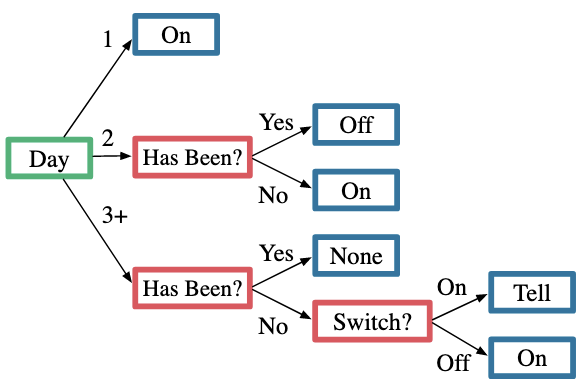
\includegraphics{images/switch_riddle}
	\caption{Image from \citet{foerster2016learning} demonstrating the learned protocol from RIAL and DIAL when each model had solved the Switch Riddle environment. The decision tree can be interpreted from a three option choice of the day outlined in green. Binary choices are outlined in red and the final action is outlined in blue. }
	\label{fig:switch_riddle_solution}
\end{figure}

Still within the cooperative setting, \citet{sukhbaatar2016commnet} assessed their model within the Traffic Junction environment which was too used in \citet{singh2018ic3net}. In this, cars enter into a grid where the they are assigned three possible routes - left, right or straight. The cars are also equipped with two actions - gas or break. If two cars collide (ie. occupy the same space in the grid) each car gets $-10$ reward and the simulation will carry. The key is that the cars have a small visibility range, but it can communicate to all cars.

\

The ideal behaviour that this environment seeks to encourage is a protocol that can broadcasts information that reduces the effect of the partial observability within the environment. Indeed, \citet{sukhbaatar2016commnet} found that the communication channel in CommNet was particularly active when agent's were in particular states, but the agents preferred not to communicate. Which gives the impression that a noisy communication channel was disruptive to the tasks and a smaller amount of clear information is more useful when solving this task. IC3Net \citep{singh2018ic3net} too used this environment and found similar results with respect to the usage of the communication channel but faster convergence to a protocol in simulations using their model.

\paragraph{Cooperative with local rewards}

\citet{peng2017bicnet} tested their model in StartCraft Combat games with local rewards. The idea with cooperation with local rewards is that global rewards structures can ignore the need for locally coordinating agents. This type of distinction is needed in a more complicated environment like StarCraft. It was found that agents were able to learn high level coordination strategies  like coordinated cover attack. The essence of cover attack is to let one agent draw fire or  attentions from the enemies, meanwhile, other agents take  advantage of this time period or distance gap to output more  harms. The difficulty of conducting cover attack lies in how  to arrange the sequential moves of multiple agents in a coordinated hit and run way. 

\paragraph{Competitive and mixed with local rewards}

IC3Net \citep{singh2018ic3net} has the advantaged of individualised rewards, unlike RIAL, DIAL \citep{foerster2016learning} and CommNet \citep{sukhbaatar2016commnet}. This means that the model can also be tested in competitive and mixed environments. \citet{singh2018ic3net} tested the model in the predator-prey environment. The environment has a fixed prey and $n$ predators. The competitiveness of the environment is adjusted based on the reward structure. In cooperative scenarios, the more predators on a prey the greater the reward, and the opposite in the competitive variation.

\

The desired communication will naturally change depending on the reward structure. In the competitive setup, one sees the communication gates (See Appendix \ref{sec:models} for details) used to reduce the communication omitted by the agents. Meaning that the model learns \textbf{not} to communicate. In the mixed environment, the use of the communication channel did not see a difference to the performance of the agents compared to a non-communicating model.  

\subsection{Communication Constraints}

Within Comm-MARL there can be constraints placed on the communication with the model and environment. These constraints are often imposed to create an analogy within real world communication. For example, typically we consider language to be communication with a finite lexicon - similar constraints are placed on communication channels to ensure only discrete communication. Communication channels can be noisy in real life and so message signals sent can also have some Gaussian noise added to it.

\paragraph{Constrained communication} DIAL and RIAL \citep{foerster2016learning} have a communication channel capacity introduced in the model. In the case of the Switch Riddle, this communication is channel is constrained to a single bit. This is a bandwidth constraint. In DIAL, we also have messages that have noise added to them - which is an example of a corrupted channel. The interesting feature of this channel is that the communication is through the noisy channel but the feedback is not. The DIAL model allows for message gradients to be passed from receiver to sender so in introducing noise to the message the agents are actually forced to be more confident in the sign\footnote{Sign in the mathematical sense of negative or positive} of the message they send.

\

Both these constraints are coupled within the model since the noise is a feature of the DRU (See Appendix \ref{subsec:dial_rial} for details) which is a device introduced to force learned protocols to be easily discretised. 

There are practical concerns that are associated with communication - such as communication costs. We can categorise the communication within this dimension as unconstrained or constrained. 

\paragraph{Unconstrained communication}
CommNet \citep{sukhbaatar2016commnet} introduces no constraint on the message that is sent. The messages are aggregations of the internals states of each agent in the environment (apart from themselves) but there is no constraint on the size of the message that is to be sent. \citet{singh2018ic3net} is similar in this unconstraint communication channel but this model has the key feature of a learnt gating mechanism of outgoing messages. This allows agents to learn not to communicate but does not have any explicit loss attached to it and is therefore not considered to be a constraint on the communication.

\subsection{Communicatee Types}

Communicatee type determines the criteria of the agent that one can send a message to. There are naturally, location constraints with communication in real life but there can be other conventions that dictate the communication within a muti-agent system. In a software development team, it is not always necessary for the developers to communicate directly with each other and could rather have a system in place where another employee is responsible for aggregating the communication from the team and passing on only what is relevant to each team member. In this case, the communication is mediated through a proxy.

\paragraph{Learning other agents to communicate with} IC3Net \citep{singh2018ic3net} have no constraint on the agents that can be communicated with. This is since all agents will be receiving an average of the hidden state of the other agents, which is the same as CommNet \citep{sukhbaatar2016commnet}. The difference is the gating introduced by \citet{singh2018ic3net} which allows agents to learn a function that can remove all communication with specific agents. 

\paragraph{Nearby agents} In NeurComm \citep{chu2020NeurComm} the MAS is represented as a graph. Where agents are considered nodes who can only communicate with their neighbours in the graph. The agent then receives their own local observation as well as the concatenation of all neighbour's messages as the ``state'' input to its neural network. For agent $i$ with a closer neighbourhood $N_i$ it would use:

\begin{equation}
	s_i^t = o_i^t \cup m_{N_i}^t 
\end{equation}

Where $m_{N_i}^t = \{ m_j^t : j \in N_i \}$.

\paragraph{Proxy} A proxy is a virtual agent that plays an essential role (e.g., as a medium) in facilitating communication but does not directly affect the environment. Using a proxy as the communicatee means that agents will not directly communicate with each other, instead viewing the proxy as a medium, coordinating and transforming messages for specific purposes. In the HAMMER model \citep{gupta2022HAMMER} there is a centralised agents that receives all observation as input to its neural network. In other words, the central agent receives $\mathbf{s^t} = [o^t_1, \hdots, o_J^t]$ with $J$ agents in the environment at time $t$. The central agent is then responsible for generating personalised messages for each agent in the form of single real number or a real-valued vector with a small number of dimensions. This proxy agent can then be trained using the gradients computed by the individual agents, or using the global rewards of the agents. This represents a differentiable vs reinforced learning scheme which will be discussed in Section \ref{sec:learning_methods}. 

\begin{figure}
	\centering
	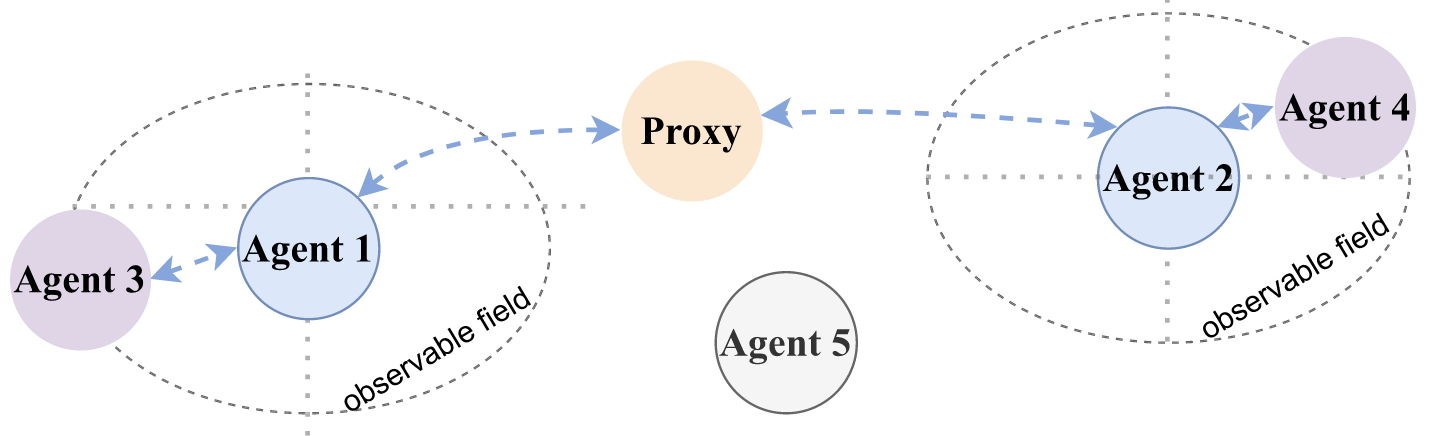
\includegraphics[scale=0.5]{images/communicatee.png}
	\caption{Image from \citet{zhu2024survey} demonstrating the difference between communication among nearby agents within the observable field, and communication between agents between a mediating proxy agent.}
	\label{fig:communicatee}
\end{figure}

\subsection{Communication policy}

%TODO: Split with global and local policies

A communication policy defines a set of communication actions, which can be modelled in different ways. For example, a communication action can be represented as a vector of binary values, where each value indicates whether communication with one of the other agents is allowed at a certain time step. These actions form communication links between pairs of agent These policies can be learned of predefined. 

\paragraph{Predefined full communication} In DIAL and RIAL \citet{foerster2016learning} the agents have full access to communicate with all other agents. When viewed as a graph - this means that each agent is connected to every other agent so any message that gets sent by one agent is broadcast to the entire network. \citet{chuster1997Bidirectional} obtains a full communication graph but through other agents. Since, the communication within this model is using recurrent connections between the hidden states of agents. Similar to recurrent connections through time, only the preceding agent is able to send a message, but the effect of the previous recurrent connection is still present in the hidden state that is being communicated. Thus, there is a sort of implicit full communication structure in this model. 

\paragraph{Learnt individual control} IC3Net \citep{singh2018ic3net} has a gating mechanism that enables the agents to learn to communicate or not to communicate with a certain agent. In this sense, their communication policy is learnt during training. A crucial point is that the learning is done individually. Each agent is tasked with performing this same task. This is in contract to other models in which a global controller determines the communication policy. 

\begin{figure}
	\centering
	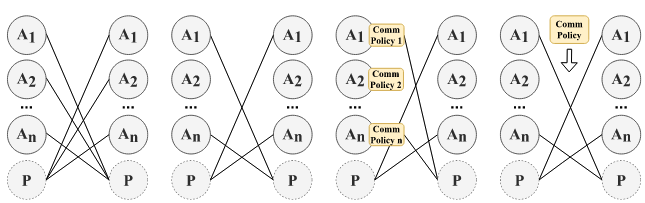
\includegraphics[scale=0.5]{images/communication_policies.png}
	\caption{\citet{zhu2024survey}}
	\label{fig:communication_policies}
\end{figure}

\subsection{Communicated messages}

After establishing communication links among agents through a communication policy, agents should determine which specific information to communicate. This information can derive from historical experiences, intended actions, or future plans, enriching the messages with valuable insights. Consequently, the communicated information can expand the agents’ understanding of the environment and enhance the coordination of their behaviors. In the dimension of communicated messages, an important consideration is whether the communication includes future information, such as intentions and plans. This kind of information, being inherently private, often requires an (estimated) model of the environment to effectively simulate and generate conjectured intentions and plans.

\paragraph{Existing knowledge} In this category agents share knowledge about their environment. This can be in the form of low dimensional encoding of their hidden states. This is particularly prevalent in models based on RNN's \citep{sukhbaatar2016commnet, peng2017bicnet, singh2018ic3net}. The architecture allows for the encoding of previous information, as well as present observation to then be combined into a message for the other agents. RIAL and DIAL \citep{foerster2016learning} have message as output in their RNN's as opposed to communicating hidden states. Intuitively, this means that messages are more explicitly learnt.

\paragraph{Imagined future knowledge} In NeurComm \citep{chu2020NeurComm} agents do not only communicate their existing knowledge but too some prediction about their future actions. Existing knowledge is communication in a similar manner to other models where the is some aggregation of the hidden states of the model that is communicated. The future knowledge that the agent passes on is in the form of a policy fingerprint. In this, the agent encodes future actions in particular states that can be used by other agents to plan their policies. The problem in this scheme is the moving target. If one agent communicated a policy finger print, that informs another agent's policy which it too communicates. This issue did not arise in NeurComm, however.


\subsection{Message combination}

When agents receive more than one message, current works often aggregate all received messages to reduce the input for the action policy. Message Combination determines how to integrate multiple messages before they are processed by an agent’s internal model. If a proxy is involved, each agent receives already coordinated and combined messages from the proxy, eliminating the need for further message combination. If no proxy is presented, each agent independently determines how to combine multiple messages. Since communicated messages encode the senders’ understanding of the learning process or the environment, some messages can be more valuable than others. 

\paragraph{Equally valued} In this category, messages received by agents are treated without preference, meaning they are assigned equal weights or simply no weights at all. Without having preferences, agents can concatenate all messages, ensuring no loss of information, though it may significantly expand the input space for the action policy. Equally values messages are found in RIAL and DIAL \citep{foerster2016learning}, CommNet \citep{sukhbaatar2016commnet} and IC3Net \citep{singh2018ic3net}. 

\paragraph{Unequally valued} In BiCNet \citep{peng2017bicnet} the message received from agents that have closer indexes will have a greater influence on the message that is being communicated. The messages in this model flow through recurrent connection in the RNN. Thus, the message sent from an agent indexed further away will have less impact on the agent's actions. Social convention-like roles emerged from these unequal weightings. For instance, certain agents might be more critical in relaying positioning information, while others may prioritise attack strategies, resulting in a form of "social convention" where some agents’ messages carry more significance in coordinating team behaviour.

\subsection{Inner Integration}

Inner Integration determines how to integrate (combined) messages into an agent’s learning model, such as a policy or a value function. In most existing literature, messages are viewed as additional observations. Agents take messages as extra input to a policy function, a value function, or both. Thus, in the dimension of inner integration, we classify recent works into categories based on the learning model that is used to integrate messages.

%CommNet, IC3Net 
\paragraph{Policy-level}
By exploiting information from other agents, each agent will no longer act independently. Policies can be learned through policy gradient methods like REINFORCE, as seen in studies \citet{sukhbaatar2016commnet, singh2018ic3net} which collect rewards during episodes and train the policy models at the end of episodes. Moreover, the Comm-MADRL approaches that utilise actor-critic methods \citep{gupta2022HAMMER} that assume that a critic model guides the learning of an actor model.

%RIAL and DIAL
\paragraph{Value-level}
In this category, a value function incorporates messages as input, and a policy is derived by selecting the action with the highest Q-value. Most works in this category employ DQN-like methods to train their value functions \citep{foerster2016learning}.

%BiCNet
\paragraph{Policy and value level}
Integrating messages using both a policy function and a value function typically relies on actor-critic methods. In Comm-MADRL approaches within this category, received messages can be treated as extra inputs for both the actor and critic models \citep{peng2017bicnet} Alternatively, messages can be combined with local observations to generate new internal states, which are then shared with both the actor and critic models.


\subsection{Learning methods}\label{sec:learning_methods}

Learning methods determine which type of machine learning techniques is used to learn a communication protocol. The learning of communication is at the centre of modern Comm-MADRL and can benefit from the advancements in the machine learning field. If proper assumptions about communication are made, such as being able to calculate the derivatives with respect to the message generator function and the communication policy, then the training of communication can be integrated into the overall learning process of agents. This integration allows for the use of fully differentiable methods for backpropagation. Other machine learning techniques, including reinforcement learning can too be used to learn the a communication protocol. 

\paragraph{Differentiable} Neural Networks are end to end differentiable which means that networks can pass gradients in order to improve the feedback mechanisms present in their communication. In DIAL \citep{foerster2016learning} the gradient of the message sent by the receiver is propagated back to the sender. This is akin to the feedback we have in human interaction where someone nods to confirm their understanding of something being said. In this set-up, the communicated type is agents. In HAMMER \citep{gupta2022HAMMER}, the communication is mediated through the a central agent. This agent can too receive the gradient feedback from each agent given the personalised message it sent. What is crucial is that all messages and computations are fully-differentiable so we are able to pass around gradients. Once there is some discontinuity, this is particularly important since models can enforce discrete communication which naturally introduces jump discontinuities. In DIAL, this is resolved using the DRU to create differentiable messaging during training and then discrete messages during execution.

\paragraph{Reinforced} Models can also use methods of reinforcement learning in order to learn communication protocols. In this case, the gradients are based on the reward feedback from the environment. In this, the messages can be seen as included in the action space for each agent. The issue in this is that the reward feedback is now a black-box - in the same way that the action to reward relationship is in regular reinforcement learning. RIAL \citep{foerster2016learning} still learned a solution policy to the three agent Switch Riddle but was not able to achieve any learning when the size of the environment increased to four agents. A similar less effective training was seen in HAMMER \citep{gupta2022HAMMER} when using reinforced learning techniques.

\subsection{Training schemes}

This dimension focuses on how to utilise the collected experiences (such as observations, actions, rewards, and messages) of agents to train their action policies and communication architectures in a Comm-MADRL system. Agents can train their models in a fully decentralised manner using only their local experience. Alternatively, when global information is accessible, the experiences of all agents can be collected to centrally train a single (centralised) model that controls all agents. However, each approach has inherent challenges. Fully decentralised learning must cope with a non-stationary environment due to the changing and adapting behaviours of agents, while fully centralised learning faces the complexities of joint observation and policy spaces. As a balanced solution, Centralised Training and Decentralised Execution (CTDE). 

\paragraph{Centralised learning and decentralised execution} In CTDE approaches, the experiences of all agents are collectively used for optimisation. Gradients derived from the joint experiences of agents guide the learning of local policies. However, once training is complete, only the policies are needed and gradients can be discarded, facilitating decentralised execution. When agents are assumed to be homogeneous, meaning they have identical sensory inputs, actuators, and model structures, they can share parameters. Parameters sharing reduces the overall number of parameters, potentially enhancing learning efficiency compared to training in separate processes. Despite sharing parameters, agents can still exhibit distinct behaviours because they are likely to receive different observations at the same time step.


\paragraph{Decentralised Learning} In decentralised learning the agent only has access to local observations and chooses actions based on these observations. Within Comm-MARL, the agents have access to messages that may communicated to them. In this sense, there may be information in those messages that is not in the immediate proximity of that agent. In NeurComm \citep{chu2020NeurComm} this training regiment is used. Where global information can be present through cascaded neighbourhood communications.

\section{Results}

\section{Conclusion}

\newpage

\bibliography{references}
\addcontentsline{toc}{section}{References}

\newpage

\appendix

\section{MARL Communication Models} \label{sec:models}
\subsection{RIAL and DIAL}\label{subsec:dial_rial}

Both \textbf{r}einforced \textbf{i}nter-\textbf{a}gent learning (RIAL) and \textbf{D}ifferentiable \textbf{i}nter-\textbf{a}gent learning (DIAL) were proposed in \citet{foerster2016learning}. These models are architecturally identical but are differentiated by the way the gradient of the parameters responsible for generating messages are computed during learning.

\

The foundations for this model are in Deep Q-Networks, Deep Recurrent Q-Networks and Independent Q-learning outlined in sections ... respectively. With a key difference being the disabling of the experience replay in the RIAL and DIAL models, since it was found that the non-stationarity of the multi-agent environment meant the agent was learning from obsolete and misleading data in the experience replay. The specific training and execution configuration considering in these models is one of centralised training and decentralising execution. What's more, is that only discrete messages are considered in these models. 


\paragraph{RIAL} Each agent's Q-network is represented by $Q^a(o_t^a, m_{t-1}^{a'}, h_{t-1}^{a}, u^a)$ which are all conditioned on the agent indexed by $a$, where $a'$ refers to the other agents. To avoid a network with output dimension $|U||M|$, the Q-network is split between the environment ($Q^a_u$) and communication ($Q^a_m$) action networks. There is then an actor selector that picks $u_t^a$ and $m_t^a$ from the q-value output using an $\varepsilon$-greedy policy. Hence, the network requires only $|U| + |M|$ outputs and action selection requires maximising over U and then over M , but not maximising over $|U| \times |M|$.

\paragraph{Parameter Sharing} RIAL can be extended to take advantage of the opportunity for centralised learning by sharing parameters among the agents. This variation learns only one network, which is used by all agents. However, the agents can still behave differently because they receive different observations and thus evolve different hidden states. In addition, each agent receives its own index a as input, allowing them to specialise.

%TODO: Need to mention the C-Net here

\paragraph{DIAL} While RIAL can share parameters among agents, it still does not take full advantage of centralised learning. In particular, the agents do not give each other feedback about their communication actions. Contrast this with human communication, which is rich with tight feedback loops. The main insight behind DIAL is that the combination of centralised learning and Q-networks makes it possible, not only to share parameters but to push gradients from one agent to another through the communication channel. Thus, while RIAL is end-to-end trainable within each agent, DIAL is end-to-end trainable across agents. Letting gradients flow from one agent to another gives them richer feedback, reducing the required amount of learning by trial and error, and easing the discovery of effective protocols. The end-to-end differentiability is violated with the discrete nature of the messages. To navigate this, \citet{foerster2016learning} propose the DRU (discretise and regularise unit) for messages to pass through before being received by other agents. The DRU has separate functions during training and execution. In training, the DRU is tasks with encouraging the agents to learn protocols that can be easily discretised. This is done by passing the message through a sigmoid activation function and to add noise. Then during execution the messages are discretise by the DRU: $DRU(m_t^a) = 1\chi_{\{ m_t^a > 0 \}}$, where $\chi$ is the indicator function.

\begin{figure}
	\centering
	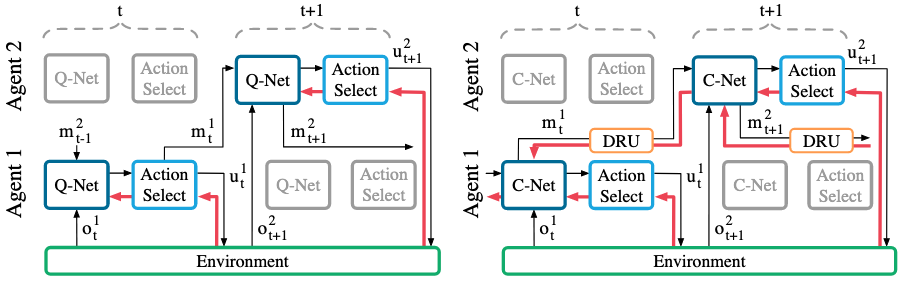
\includegraphics[scale=0.5]{images/rial_dial.png}
	\caption{Image from \citet{foerster2016learning} depicting the RIAL and DIAL model architectures with inputs and messages depicted using a black arrow and gradients depicted with red arrows. (Left) RIAL model where gradients are computed with respect to the feedback from the environment. (Right) DIAL model using the DRU that all messages pass through, as well as the direct gradient sharing between agents which uses parameter sharing.}
\end{figure}

The architecture used in both RIAL and DIAL models is identical. As illustrated in Figure \ref{fig:rial_dial_nn}, each agent is composed of a recurrent neural network (RNN), unrolled over \( T \) time-steps, which maintains an internal state \( h \). This architecture includes an input network for generating a task embedding \( z \), as well as an output network for producing Q-values and messages \( m \). The input for agent \( a \) is specified as a tuple \( (\mathbf{o}_t^a, m_{t-1}^{a'}, u_{t-1}^a, a) \). Here, the components \( a \) and \( u_{t-1}^a \) are processed through lookup tables, while \( m_{t-1}^{a'} \) is processed via a 1-layer MLP, each generating embeddings of size 128. The observation \( \mathbf{o}_t^a \) is passed through a task-specific network that generates an additional embedding of the same size. The final state embedding is then produced by the element-wise summation of these embeddings:

$$
\mathbf{z}_t^a = (\text{TaskMLP}(\mathbf{o}_t^a) + \text{MLP}[|M|, 128](m_{t-1}) + \text{Lookup}(u_{t-1}^a) + \text{Lookup}(a)).
$$

The original authors observed improved performance and stability when batch normalisation \citep{ioffe2015batch} was applied to \( m_{t-1} \) before processing. The combined embedding \( \mathbf{z}_t^a \) is subsequently processed through a 2-layer RNN with GRUs:

$$
h_{1, t}^a = \text{GRU}[128, 128](\mathbf{z}_t^a, h_{1, t-1}^a),
$$

serving as an approximation of the agent’s action-observation history. Finally, the output \( h_{2, t}^a \) from the top GRU layer is fed into a 2-layer MLP to produce both the Q-values and the message:

$$
\mathbf{Q}_t^a, \mathbf{m}_t^a = \text{MLP}[128, 128, (|U| + |M|)](h_{2, t}^a).
$$


\begin{figure}
	\centering
	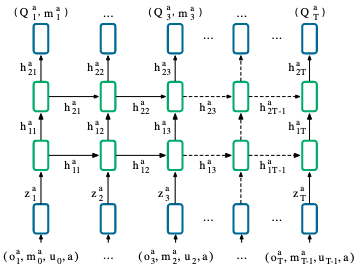
\includegraphics[scale=0.7]{images/rial_dial_nn.png}\
	\caption{Architecture of the RIAL and DIAL models from \citet{foerster2016learning}. Each agent comprises a recurrent neural network (RNN) unrolled over \( T \) time-steps, which maintains an internal state \( h \). Inputs, including observations \( \mathbf{o}_t^a \), previous messages \( m_{t-1}^{a'} \), previous actions \( u_{t-1}^a \), and agent identity \( a \), are embedded and combined to produce a state embedding \( \mathbf{z}_t^a \). The embedding is processed through a 2-layer RNN with GRUs to approximate the agent’s action-observation history. The output is then passed through a 2-layer MLP to generate both the Q-values and the message \( \mathbf{m}_t^a \).}
	\label{fig:rial_dial_nn}
\end{figure}

\subsection{CommNet}

\citet{sukhbaatar2016commnet} propose the communication neural network (CommNet) model which is centred around the global controller, $\Phi$, that is used for the computation of the actions as well as the computation of the messages. The controller maps the concatenation of all states at a point in time, $\mathbf{s} = \{ s_1, \hdots, s_J \}$\footnote{Time index is omitted for brevity}, to the concatenation of all actions, $\mathbf{a} = \{ a_1, \hdots, a_J \}$, for $J$ agents. Thus, $\mathbf{a} = \Phi(\mathbf{s})$. 

\

The structure of the controller is of the form of a neural network comprised of modules, $f^i$, for each communication step $i$. The modules take as input the hidden state $h^i_j$ and the communication $c^i_j$,  and outputs a vector $h^{i+1}_j$. The main body of the model then takes as input the concatenated vectors $\mathbf{h}^i = [h^i_1, \hdots,  h^i_J]$, and computes:

\begin{align*}
	h_j^{i+1} &= f^i(h^i_j, c^i_j) \\
	c_j^{i+1} &= \frac{1}{1 - J} \sum_{j' \neq j} h_{j'}^{i + 1}
\end{align*}

$f^i$ is a single layer neural network with a non-linearity $\sigma$. In which case, $f^i(h^i_j, c^i_j) = \sigma(H^i h^i_j +  C^i c^i_j)$. 

At the first layer of the model an encoder function $h_j^0 = r(s_j)$ is used. This takes as input state-view $s_j$ and outputs feature vector $h_j^0$ (in $R_{d_0}$ for some $d_0$). The form of the encoder is problem dependent,  but for most of our tasks it is a single layer neural network. Unless otherwise noted, $c_j^0 = 0$ for all j.  At the output of the model, a decoder function $q(h_j^K)$ is used to output a distribution over the space of  actions. $q(\cdot)$ takes the form of a single layer network, followed by a softmax. To produce a discrete  action, we sample from this distribution: $a_j \sim q(h_j^K )$.  Thus the entire model (shown in Figure \ref{fig:commnet})takes the state-view of all agents s, passes it through the encoder $h0 = r(s)$, (ii) iterates $h$ and $c$ to obtain $h^K$, (iii) samples actions $a$ for all agents, according to $q(h^K)$.

%TODO: Caption below 
\begin{figure}
	\centering
	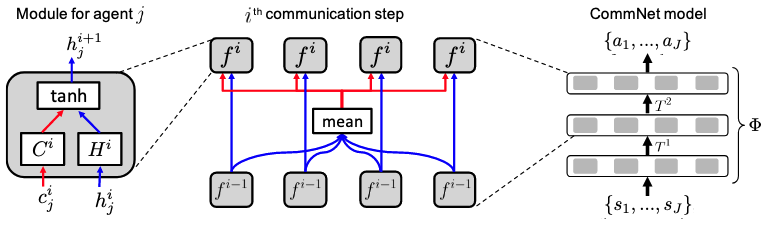
\includegraphics[scale=0.5]{images/commnet.png}
	\caption{Image from \citet{sukhbaatar2016commnet}}
	\label{fig:commnet}
\end{figure}

\subsection{IC3Net}

Individualized Controlled Continuous Communication Model (IC3Net) is a model proposed by \citet{singh2018ic3net} and represents an extension to the CommNet model \citep{sukhbaatar2016commnet}. The model is novel in that it is proposed to work in a competitive, mixed and cooperative environment by using a gating mechanism in order to determine whether to block communication between agents. In this sense the model is also learning when to communicate, as well as what to communicate.

%TODO: Caption below 
\begin{figure}
	\centering
	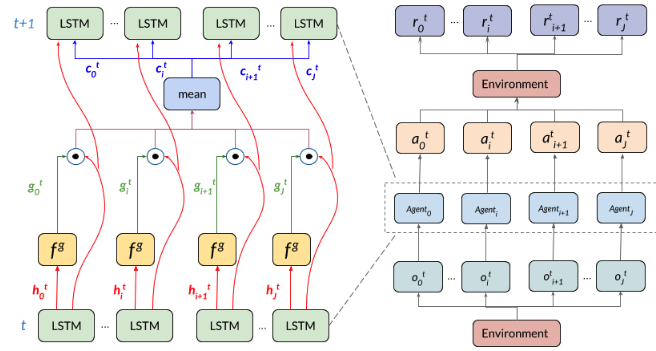
\includegraphics[scale=0.5]{images/ic3net.png}
	\caption{Image from \citet{singh2018ic3net} highlighting the architecture of of the IC3Net.}
	\label{fig:ic3net.png}
\end{figure}


IC3Net is based on an independent controller model where each agent is controlled by an individual LSTM. For the $j-th$ agent, its policy takes the form of:

\begin{align*}
h_j^{t + 1} &= LSTM(e(o_j^t), h_j^t, s_j^t)
a^t_j &= \pi(h^t_j)
\end{align*}

where $o_j^t$ is the observation of the $j-th$ agent at time $t$, $e(\cdot)$ is an encoder function parameterised by a fully-connected neural network and π is an agent’s action policy. Also, $h^t_j$ and $s^t_j$ are the hidden and cell states of the LSTM. We use the same LSTM model for all agents, sharing their parameters. IC3Net extends the independent controller model by allowing agents to communicate their internals states, gated by discrete action. The policy of the $j-th$ agent is given by:

\begin{align*}
    g_j^{t+1} &= f^g\left(h_j^t\right) \\
    h_j^{t+1}, s_j^{t+1} &= \text{LSTM}\left(e\left(o_j^t\right) + c_j^t, h_j^t, s_j^t\right) \\
    c_j^{t+1} &= \frac{1}{J-1} C \sum_{j' \neq j} h_{j'}^{t+1} \odot g_{j'}^{t+1} \\
    a_j^t &= \pi\left(h_j^t\right)
\end{align*}

where $c^t_j$ is the communication vector for the $j-th$ agent, $C$ is a linear transformation matrix for transforming gated average hidden state to a communication tensor, $J$ is the number of alive agents currently present in the system and $f^g(\cdot)$ is a simple network containing a soft-max layer for 2 actions (communicate or not) on top of a linear layer with non-linearity. The binary action $g^t_j$ specifies whether agent $j$ wants to communicate with others, and act as a gating function when calculating the communication vector. Note that the gating action for next time-step is calculated at current time-step. The action policy $\pi$ and the gating function $f^g$ with REINFORCE \cite{williams1992simple}.


\subsection{BiCNet}

Multiagent Bidirectionally-Coordinated Net (BiCNet) is a model that leverages a bidirectional Recurrent Neural Network (bi-RNN) \citep{chuster1997Bidirectional}. The model was proposed in \citet{peng2017bicnet} and facilitates information exchange between agents to improve the efficacy and efficiency of the learned communication protocol. Each agent has its own ``policy'' (actor) and ``Q'' (critic) network for learning actions and state values, respectively, and both use bi-RNNs to enable communication between agents.

\

\begin{figure}
	\centering
	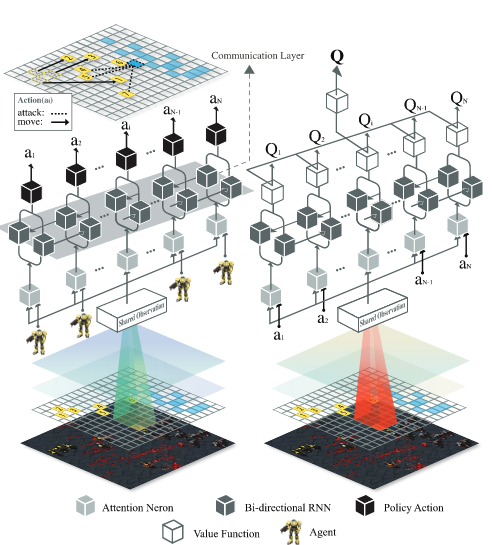
\includegraphics[scale=0.5]{images/bicnet}
	\caption{Image from \citet{peng2017bicnet} highlighting the architecture of of the BiCNet.}
	\label{fig:ic3net.png}
\end{figure}

BiCNet shares parameters across agents to ensure that the model is compact and scalable, allowing it to handle varying numbers of agents without needing retraining. This parameter-sharing mechanism is similar to RNNs, where parameters are shared across time steps. Each agent’s internal state and observed information are shared bidirectionally with other agents, promoting effective communication. By using bi-RNNs, BiCNet is not restricted to symmetric communication, enabling roles and priorities among agents, which aids in collaborative strategies.

\

Training employs backpropagation through time (BPTT) over the bi-RNN structure, calculating gradients jointly across the actor and critic networks. Specifically:

\begin{itemize}
    \item \textbf{Actor Gradient:} A multi-agent deterministic policy gradient is applied to optimise the actor, where each agent’s policy is collectively learned across agents, leading to aggregate reward optimisation.
    
    \item \textbf{Critic Gradient:} A squared loss gradient is used to optimise the critic network, where each agent’s Q-values are evaluated based on the reward and expected future reward.
    
    \item \textbf{Experience Replay:} The model uses experience replay to stabilise training, storing past interactions and sampling mini-batches to train the networks iteratively. This replay allows the agents to learn effectively from past experience rather than only recent events.
    
    \item \textbf{Exploration with Ornstein-Uhlenbeck Process:} To add stochasticity during training, the model applies noise to the actor's actions, facilitating better exploration, especially in continuous action spaces.
\end{itemize}

\textbf{Message Encoding through Hidden States:} In BiCNet, communication occurs through hidden states passed between agents in the bi-RNN layers. This process allows each agent to integrate information from others and decide actions based on both local and shared states.

\subsection{NeurComm}

NeurComm \citep{chu2020NeurComm} is a communication model that exploits the spatiotemporal dimension of the MARL problem. The Markov property is then assumed to be present in both the spatial and temporal dimensions. All messages sent from agent $i$ in this model are assumed to be equal: $m_{ij} = m_i, \ \forall j \in \mathcal{N}_i$. Then:

\begin{equation}
	h_{i, t} = g_{\nu_i} (h_{i, t-1}, e_{\lambda_i^s}(s_{\mathcal{V}_i, t}), e_{\lambda_i^p}(\pi_{\mathcal{N}_i, t-1}), e_{\lambda_i^h}(h_{\mathcal{N}_i, t-1}))
\end{equation}

Where $h_{i, t}$ is the hidden state of agent $i$ at time $t$. $e_{\lambda_i}$ and $g_{\nu_i}$ are differentiable message encoding and extracting functions. To avoid dilution of state and policy information (the former is for improving observability while the later is for reducing non-stationarity), state and policy are explicitly included in the message besides agent belief. This means:

\begin{equation}
	m_{i,t} = s_{i,t} \cup \pi_{i,t−1} \cup h_{i,t−1}
\end{equation}

The communication phase is prior-decision, so only $h_{i,t−1}$ and $\pi_{i,t−1}$ are available.

\begin{figure}
	\centering
	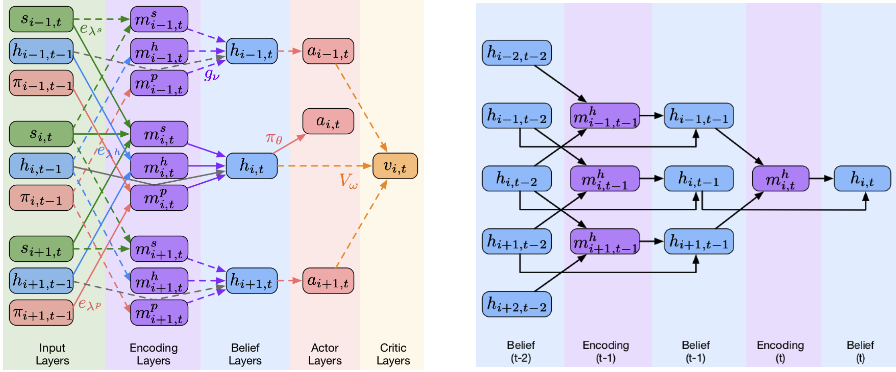
\includegraphics[scale=0.5]{images/neurcomm}
	\caption{Image from \citet{chu2020NeurComm} highlighting the architecture of of the NeurComm.}
	\label{fig:neurcomm}
\end{figure}

\subsection{HAMMER}

The Heterogeneous Agents Mastering Messaging to Enhance Reinforcement learning (HAMMER) \citep{gupta2022HAMMER} presents an architecture based on independent learners and a global learner. The independent learners are the agents performing actions in the environment, while the central learner serves as a proxy for generating messages that aid coordination among these agents.

\

At the start of each time step, the central agent receives the observations of all agents, denoted as $\mathbf{s^t} = [o_1^t, \hdots, o_j^t]$, where $o_j^t$ represents the observation of agent $j$ at time $t$. The central agent processes this combined observation and outputs a personalized message $m_i^t$ for each agent $i$. Each independent agent then combines its local observation $o_i^t$ with the received message $m_i^t$ to inform its action selection within the environment. These dynamics are illustrated in Figure \ref{fig:hammer}.

\begin{figure}
	\centering
	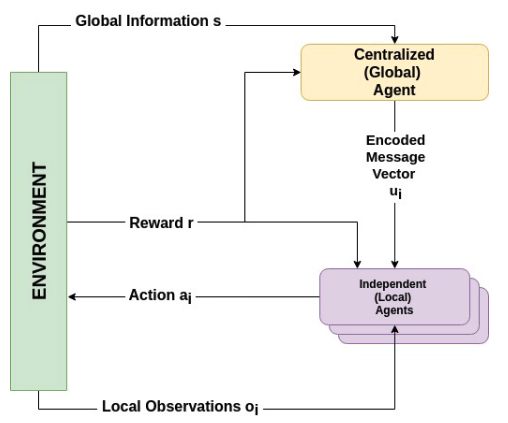
\includegraphics[scale=0.5]{images/hammer}
	\caption{Image from \citet{gupta2022HAMMER} depicting the information exchange of the HAMMER model during a single time-step.}
	\label{fig:hammer}
\end{figure}

\

The independent agents implement Proximal Policy Optimisation (PPO) \citep{schulman2017proximal} as their reinforcement learning model. To ensure consistent policy updates and computational efficiency, the independent agents use \textit{parameter sharing}, where a single network with shared parameters represents the policies of all agents. This shared network structure enables experience collected by each agent to contribute toward updating a common policy.

\

To further stabilise training, HAMMER employs \textit{experience replay} with two separate memory buffers: one for the independent agents and one for the central agent. The replay buffers store experiences, allowing the central and independent agents to sample past interactions during updates. This approach enhances sample efficiency and reduces variance in the learning process.

\

During training, gradients are computed with respect to both the actions chosen by each independent agent and the parameters associated with the message input from the central agent. By back-propagating these gradients through the network, the central agent’s message-generation process is fully differentiable, allowing it to adapt its messaging strategy dynamically based on feedback from the agents’ learning. Additionally, the central agent can utilise the global reward signal, aggregating the outcomes of the independent agents' actions, to further refine the message content it sends, thereby optimising coordination in the environment.

\end{document}






























